
%----------------------------------------------------------------------------------------
%	PART
%----------------------------------------------------------------------------------------


\part{Capítulo ocho}

%Esto para no tener que escribir toda la ruta en cada magen agregada
\graphicspath{{W_Varios/2_Portada_capitulos/},{8_Capitulo/ejemplos/} }

%----------------------------------------------------------------------------------------
%	CHAPTER 8
%----------------------------------------------------------------------------------------



%----------------------------------------------------------------------------------------
%	PART
%----------------------------------------------------------------------------------------


\graphicspath{{W_Varios/2_Portada_capitulos/},{8_Capitulo/ejemplos/} }

%----------------------------------------------------------------------------------------
%	CHAPTER 8
%----------------------------------------------------------------------------------------



%----------------------------------------------------------------------------------------
%	PART
%----------------------------------------------------------------------------------------


\chapter{Formulación de funciones financieras en Excel}

\section{Fórmulas del capítulo/Excel Financiero}

\vspace{2mm}

\begin{center}
 \begin{tabular}{ |p{8cm}| p{5cm}|}
  \hline
  \rowcolor{orange!50}
  \begin{center}\textbf{Nombre} \end{center}              & \begin{center} \textbf{Función Financiera en Excel} \end{center} \\ \hline

  Equivalencia de tasas periódicas       & TASA(m;;-1;1+i)           \\\hline

  Tasa interés nominal anual vencida     & TASA.NOMINAL(i;m)         \\ \hline

  Tasa interés periódica año vencido     & INT.EFECTIVO(j;m)         \\ \hline

  Valor futuro                           & VF(i;n;;VA,0)             \\ \hline

  Valor presente                         & VA(i;n;;VF,0)             \\ \hline

  Valor presente serie uniforme vencida  & VNA(i;R1;R2;R3;...)       \\ \hline

  Valor futuro serie uniforme vencida    & VF(i;n;;VA,0)             \\ \hline

  Valor futuro serie uniforme anticipada & VF(i;n;;VA,1)             \\ \hline

  Valor presente serie perpetua vencida  & VA(i;n;R;0)               \\ \hline

  Valor presente gradiente aritmético    & VNA(i;R1;R2;R3;...)       \\ \hline

  Valor presente gradiente geométrico    & VNA(i;R1;R2;R3;...)       \\ \hline

  Valor cuota serie uniforme vencida     & PAGO(i;n;P;F;0)           \\ \hline

  Valor cuota serie uniforme anticipada  & PAGO(i;n;P;F;1)           \\ \hline

  Ecuación de valor                      & Función Buscar Objetivo   \\ \hline
 \end{tabular}
\end{center}

\clearpage

\section{Introducción}

En este capítulo veremos la forma de resolver ejercicios de Ingeniería Económica mediante el uso del ordenador, más específicamente usando el programa de Excel, mediante la implementación de las funciones financieras que este nos brinda, para esto es importante consultar la Guía para resolver ejercicios de Ingeniería Económica a partir de Excel financiero y el uso de funciones financieras en Excel presentes en el inicio de la guía ya que este ofrecerá la metodología que debe ser aplicada para la correcta resolución de los ejercicios, además de presentar en esta las funciones que pueden ser aplicadas dando una explicación de estas y mostrando donde pueden ser aplicadas.
\\

Es importante resaltar las ventajas que ofrece la resolución de los ejercicios por este método: \\

\begin{itemize}
 \item Eficiencia en cuanto a la resolución de los ejercicios es mayor.\\
 \item Se reduce la fuente del error que se puede llegar a obtener en el ejercicio ya que no es necesario la aplicación de cálculos a mano o en calculadora ya que todo es realizado por Excel.\\
 \item Mejora la presentación del ejercicio.\\
 \item Permite realizar un análisis de sensibilidad que por otro método no es posible.\\

\end{itemize}

Para mostrar las ventajas que posee el uso de Excel a continuación se mostraran diversos ejemplos sobre los diferentes temas tomados de los capítulos 2, 4, 5, 6 y 7 presentes en la Guía de Ingeniería Económica.

\section{Ejemplos}

\textbf{Ejemplo 1}\\
Para realizar un proyecto se necesita realizar una inversión inicial de 80.000 COP y otra inversión de
45.000 COP al final del primer mes, en los meses 2 y 3 los ingresos son equivalentes a los egresos;
pero a partir del mes 4, se producen ingresos así: Mes cuatro 30.000 COP, mes cinco 50.000 COP, mes
seis 60.000 COP. Determinar si el proyecto lo pueden realizar los inversionistas A o B mencionados
anteriormente.\\


%%%%%%%%%%%%%%%%%%% EJERCICIO 1 %%%%%%

%\newpage %USAR SOLO SI EL SOLUCION QUEDA SOLO Y ES NECESARIO BAJARLO A LA SIGUIENTE PAGINA
\textbf{Solución.}\\
%La tabla ira centrada
\begin{center}
	\renewcommand{\arraystretch}{1.5}% Margenes de las celdas
	%Creacion de la cuadricula de 3 columnas \end{flushleft}
	\begin{longtable}[H]{|C{0.3\linewidth}|C{0.3\linewidth}|C{0.3\linewidth}|}
		%Creamos una linea horizontal
		\hline
         %%%%% INICIO FLUJO DE CAJA
		\rowcolor[HTML]{FFB183}
		\multicolumn{3}{|c|}{\cellcolor[HTML]{FFB183}\textbf{1. Asignación periodo focal}}   \\ \hline
		\multicolumn{3}{|c|} {$pf = 0 pmv$} \\ \hline
		%%%%%%%%%% FIN TITULO
		%%%%%%%%%% INICIO TITULO
		%Lo que se hace aqui es mezclar las 3 columnas en una sola
		\multicolumn{3}{|c|}{\cellcolor[HTML]{FFB183}\textbf{2. Declaración de variables}}   \\ \hline
		%%%%%%%%%% FIN TITULO
		%%%%%%%%%% INICIO DE MATEMATICAS
		%Cada & hace referencia al paso de la siguiente columna
		$n_{0} = 0 pmv$   & $n_{1} = 1 pmv$ & $n_{2} =  4 pmv$\\
		$n_{3} = 5 pmv$ & $n_{4} = 6 pmv$ & \\ \hline
		\multicolumn{3}{|c|}{$i_{a} = TIO_{a} = 3\% \equiv 0.03 pmv$} \\
		\multicolumn{3}{|c|}{$i_{b} = TIO_{b} = 2\% \equiv 0.02 pmv$} \\ \hline
		%%%%%%%%%% FIN DE MATEMATICAS
		%%%%% FIN DECLARACION DE VARIABLES


		%%%%% INICIO FLUJO DE CAJA
		\rowcolor[HTML]{FFB183}
		\multicolumn{3}{|c|}{\cellcolor[HTML]{FFB183}\textbf{3. Diagrama de flujo de caja}} \\ \hline
		%Mezclamos 3 columnas y ponermos el dibujo
		%%%%%%%%%%%%% INSERCION DE LA IMAGEN
		%Deberan descargar las imagenes respectivas del drive y pegarlas en la carpeta
		%n_capitulo/img/ejemplos/1/capitulo1ejemplo1.pdf  (el /1/ es el numero del ejemplo)
		\multicolumn{3}{|c|}{ 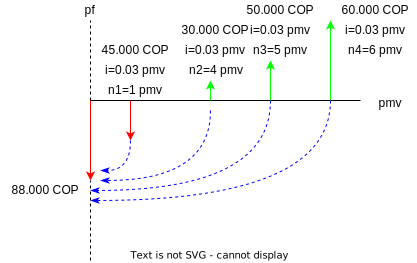
\includegraphics[trim=-5 -5 -5 -5 , scale=1.0,width=300px, height=250px]{9_Capitulo/ejemplos/1/Capitulo9Ejercicio1.pdf} }   \\ \hline
		%%%%%%%%%%%%% FIN INSERCION DE IMAGEN
		%%%%%FIN FLUJO DE CAJA



		%%%%% INICIO DECLARACION FORMULAS
		%%%%%%%%%%% INICIO TITULO
		\rowcolor[HTML]{FFB183}
		\multicolumn{3}{|c|}{\cellcolor[HTML]{FFB183}\textbf{4. Declaración de fórmulas}}    \\ \hline
		%%%%%%%%%%% FIN TITULO
		%%%%%%%%%%% INICIO MATEMATICAS
		\multicolumn{3}{|c|}{$\sum F_{n}(1+i)^{-n} $\hspace{0.3cm} \textit{Valor presente neto}} \\ \hline
		%%%%%%%%%% FIN MATEMATICAS
		%%%%%% INICIO DESARROLLO MATEMATICO
		\rowcolor[HTML]{FFB183}
		%%%%%%%%%%INICIO TITULO
		\multicolumn{3}{|c|}{\cellcolor[HTML]{FFB183}\textbf{5. Desarrollo matemático}}       \\ \hline
		%%%%%%%%%% FIN TITULO
		%%%%%%%%%% INICIO MATEMATICAS
		\multicolumn{3}{|c|}{$VPN_{a} = -80000 - 45000(1+0.03)^{-1} + 30000(1+0.03)^{-4} + 50000(1+0.03)^{-5} + 60000(1+0.03)^{-6}$} \\
		\multicolumn{3}{|c|}{$VPN_{a} = -3655$} \\
		\multicolumn{3}{|c|}{$VPN_{b} = -80000 - 45000(1+0.02)^{-1} + 30000(1+0.02)^{-4} + 50000(1+0.02)^{-5} + 60000(1+0.02)^{-6}$} \\
		\multicolumn{3}{|c|}{$VPN_{b} = 216254$} \\ \hline

		%%%%%%%%%% FIN MATEMATICAS
		%%%%%% FIN DESARROLLO MATEMATICO
		%%%%%% INICIO RESPUESTA
		\rowcolor[HTML]{FFB183}
		%%%%%%%%%%INICIO TITULO
		\multicolumn{3}{|c|}{\cellcolor[HTML]{FFB183}\textbf{6. Respuesta}}   \\ \hline
		%%%%%%%%%% FIN TITULO
		%%%%%%%%%% INICIO RESPUESTA MATEMATICA
		\multicolumn{3}{|c|}{Para B el $VPN > 0$, significa que puede realizar el proyecto en pesos de hoy,} \\ 
		\multicolumn{3}{|c|}{además de ganarse el 2\%, obtiene una ganancia de 2.162,54 COP.}  \\ \hline
		%%%%%%%%%% FIN MATEMATICAS
		%%%%%% FIN RESPUESTA
	\end{longtable}
	%Se crean dos lineas en blanco para que no quede el siguiente texto tan pegado
	%\newline \newline %USARLO SI CREES QUE ES NECESARIO
\end{center}
%%%%%%%%%%%%%%%%%%%%%%%%%%FIN EJERCICIO 1 %%%%%%%%%%%%%%%%%%%%%%%%%%%

\textbf{Ejemplo 2}\\
Se invierten 200{.}000 COP en un depósito a término fijo de 6 meses en un banco que paga el 28\% namv. Determinar el monto de la entrega al vencimiento.\\

%%%%%%%%%%%%%%%%%%% EJERCICIO 1 %%%%%%

%\newpage %USAR SOLO SI EL SOLUCIÓN QUEDA SOLO Y ES NECESARIO BAJARLO A LA SIGUIENTE PAGINA
\textbf{Solución.}
%La tabla ira centrada
\begin{center}
  \renewcommand{\arraystretch}{1.5}% Margenes de las celdas
  %Creación de la cuadricula de 3 columnas \end{flushleft}
  \begin{longtable}[H]{|C{0.3\linewidth}|C{0.3\linewidth}|C{0.3\linewidth}|}
    %Creamos una linea horizontal
    \hline
    %Definimos el color de la primera fila
    \rowcolor[HTML]{FFB183}
    %%%%% INICIO ASIGNACIÓN FECHA FOCAL %%%%%%%
    %%%%%%%%%% INICIO TITULO
    %Lo que se hace aquí es mezclar las 3 columnas en una sola
    \multicolumn{3}{|c|}{\cellcolor[HTML]{FFB183}\textbf{1. Asignación período focal}}                                  \\ \hline
    %%%%%%%%%% FIN TITULO
    %%%%% INICIO DECLARACIÓN DE VARIABLES %%%%%%%
    \multicolumn{3}{|c|}{$pf = 6pmv$}                                                                                   \\ \hline
    %%%%%%%%%% INICIO TITULO
    %Lo que se hace aquí es mezclar las 3 columnas en una sola
    \multicolumn{3}{|c|}{\cellcolor[HTML]{FFB183}\textbf{2. Declaración de variables}}                                  \\ \hline
    %%%%%%%%%% FIN TITULO
    %%%%%%%%%% INICIO DE MATEMÁTICAS
    %Cada & hace referencia al paso de la siguiente columna
    $P =  200{.}000$ COP & $n = 6\textit{pmv} $ & $i= ?\% pmv$                                                           \\
    $j=28\%namv$         & $m=12pmv$            & $F = ? COP$                                                           
    \\\hline

    %%%%%%%%%% FIN DE MATEMÁTICAS
    %%%%% FIN DECLARACIÓN DE VARIABLES


    %%%%% INICIO FLUJO DE CAJA
    \rowcolor[HTML]{FFB183}
    \multicolumn{3}{|c|}{\cellcolor[HTML]{FFB183}\textbf{3. Diagrama de flujo de caja}}                                 \\ \hline
    %Mezclamos 3 columnas y pondremos el dibujo
    %%%%%%%%%%%%% INSERCIÓN DE LA IMAGEN
    %Deberán descargar las imágenes respectivas del drive y pegarlas en la carpeta
    %n_capitulo/img/ejemplos/1/capitulo1ejemplo1.pdf  (el /1/ es el numero del ejemplo)
    \multicolumn{3}{|c|}{ 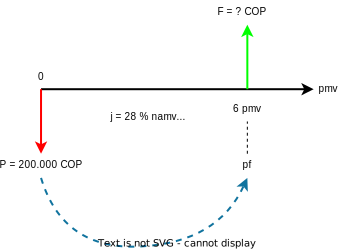
\includegraphics[trim=-5 -5 -5 -5 , scale=1]{2_Capitulo/ejemplos/2/Capitulo2Ejercicio2_v2.pdf} } \\ \hline
    %%%%%%%%%%%%% FIN INSERCIÓN DE IMAGEN
    %%%%%FIN FLUJO DE CAJA



    %%%%% INICIO DECLARACIÓN FORMULAS
    %%%%%%%%%%% INICIO TITULO
    \rowcolor[HTML]{FFB183}
    \multicolumn{3}{|c|}{\cellcolor[HTML]{FFB183}\textbf{4. Declaración de fórmulas}}                                   \\ \hline
    %%%%%%%%%%% FIN TITULO
    %%%%%%%%%%% INICIO MATEMÁTICAS
    \multicolumn{3}{|c|}{$F = P(1+i)^n \hspace{0.3cm} \textit{Valor futuro}$}                                           \\
    \multicolumn{3}{|c|}{$j=i\cdot m\hspace{0.3cm}\textit{Tasa periódica anualizada}$}
    \\ \hline
    %%%%%%%%%% FIN MATEMÁTICAS
    %%%%%% INICIO DESARROLLO MATEMÁTICO
    \rowcolor[HTML]{FFB183}
    %%%%%%%%%%INICIO TITULO
    \multicolumn{3}{|c|}{\cellcolor[HTML]{FFB183}\textbf{5. Desarrollo matemático}}                                     \\ \hline
    %%%%%%%%%% FIN TITULO
    %%%%%%%%%% INICIO MATEMÁTICAS
    \multicolumn{3}{|c|}{$0{.}28=i\cdot 12$}                                                                            \\
    \multicolumn{3}{|c|}{$i= \frac{0{.}28}{12} = 0{.}02333... \equiv 2{.}333\%pmv$}                                     \\
    \multicolumn{3}{|c|}{$0{.}28=i\cdot 12$}                                                                            \\
    \multicolumn{3}{|c|}{$F = 200{.}000 COP(1+0,2333)^6$}                                                       \\
    \multicolumn{3}{|c|}{$F = 229{.}685.04 COP$}
    \\ \hline


    %%%%%%%%%% FIN MATEMÁTICAS
    %%%%%% FIN DESARROLLO MATEMÁTICO
    %%%%%% INICIO RESPUESTA
    \rowcolor[HTML]{FFB183}
    %%%%%%%%%%INICIO TITULO
    \multicolumn{3}{|c|}{\cellcolor[HTML]{FFB183}\textbf{6. Respuesta}}                                                 \\ \hline
    %%%%%%%%%% FIN TITULO
    %%%%%%%%%% INICIO RESPUESTA MATEMÁTICA
    \multicolumn{3}{|c|}{$F = 229{.}685.04 COP$
    }                                                                                                                   \\ \hline
    %%%%%%%%%% FIN MATEMÁTICAS
    %%%%%% FIN RESPUESTA
  \end{longtable}
  %Se crean dos lineas en blanco para que no quede el siguiente texto tan pegado
  %\newline \newline %USARLO SI CREES QUE ES NECESARIO
\end{center}
%%%%%%%%%%%%%%%%%%%%%%%%%%FIN EJERCICIO 1 %%%%%%%%%%%%%%%%%%%%%%%%%%%

\textbf{Ejemplo 3}\\
Una fabrica produce actualmente en forma manual 1.000 unidades de un determinado artículo, para ello utiliza artesanos a los cuales les paga 8.400.000 COP al año y, es costumbre que cada año se les aumente el sueldo en aproximadamente un 20\%. El precio de venta de cada artículo es de 9.000 COP y se estima que este precio podrá ser aumentado todos los años en un 21\%. Ahora se ha presentado la oportunidad de adquirir una máquina a un costo de 10 millones COP con una vida útil de 5 años; un valor de salvamento de 2 millones COP la cual requiere de 2 técnicos para su operación, el sueldo anual de cada uno de los técnicos puede ser de 600.000 COP con aumentos anuales de sueldo del 20\% ¿Cuál de las dos alternativas es mejor suponiendo que la tasa del inversionista es del 30\%?\\


%%%%%%%%%%%%%%%%%%% EJERCICIO 3 %%%%%%

%\newpage %USAR SOLO SI EL SOLUCION QUEDA SOLO Y ES NECESARIO BAJARLO A LA SIGUIENTE PAGINA
\textbf{Solución.}\\
%La tabla ira centrada
\begin{center}
	\renewcommand{\arraystretch}{1.5}% Margenes de las celdas
	%Creacion de la cuadricula de 3 columnas \end{flushleft}
	\begin{longtable}[H]{|C{0.3\linewidth}|C{0.3\linewidth}|C{0.3\linewidth}|}
		%Creamos una linea horizontal
		\hline
        %%%%% INICIO FLUJO DE CAJA
		\rowcolor[HTML]{FFB183}
		\multicolumn{3}{|c|}{\cellcolor[HTML]{FFB183}\textbf{1. Asignación periodo focal}}   \\ \hline
		\multicolumn{3}{|c|} {$pf = 0 pav$} \\ \hline
		%%%%%%%%%% FIN TITULO
		%%%%%%%%%% INICIO TITULO
		%Lo que se hace aqui es mezclar las 3 columnas en una sola
		\multicolumn{3}{|c|}{\cellcolor[HTML]{FFB183}\textbf{2. Declaración de variables}}   \\ \hline
		%%%%%%%%%% FIN TITULO
		%%%%%%%%%% INICIO DE MATEMATICAS
		%Cada & hace referencia al paso de la siguiente columna
		$R_{1} = 9.000.000 $ COP   & $R_{2} = 8.400.000$ COP  & $i=0.3pav$\\ 
		$g_{1} =  0.21 pav $ & $g_{2}=  0.2 pav $ & $n=5pav$ \\ \hline
		%%%%%%%%%% FIN DE MATEMATICAS
		%%%%% FIN DECLARACION DE VARIABLES

  		%%%%% INICIO DECLARACION FORMULAS
  
		%%%%%%%%%%% INICIO TITULO
		\rowcolor[HTML]{FFB183}
		\multicolumn{3}{|c|}{\cellcolor[HTML]{FFB183}\textbf{3. Diagrama de flujo de caja}} \\ \hline
		%Mezclamos 3 columnas y ponermos el dibujo
		%%%%%%%%%%%%% INSERCION DE LA IMAGEN
		%Deberan descargar las imagenes respectivas del drive y pegarlas en la carpeta
		%n_capitulo/img/ejemplos/1/capitulo1ejemplo1.pdf  (el /1/ es el numero del ejemplo)
		\multicolumn{3}{|c|}{ \includegraphics[trim=-5 -5 -5 -5 , scale=1, width=300px, height=250px]{9_Capitulo/ejemplos/3/Capitulo9Ejercicio3.pdf} }   \\ \hline
		%%%%%%%%%%%%% FIN INSERCION DE IMAGEN
		%%%%%FIN FLUJO DE CAJA



		%%%%% INICIO DECLARACION FORMULAS
		%%%%%%%%%%% INICIO TITULO
		\rowcolor[HTML]{FFB183}
		\multicolumn{3}{|c|}{\cellcolor[HTML]{FFB183}\textbf{4. Declaración de fórmulas}}    \\ \hline
		%%%%%%%%%%% FIN TITULO
		%%%%%%%%%%% INICIO MATEMATICAS
		\multicolumn{3}{|c|}{$\sum F_{n}(1+i)^{-n} $\hspace{0.3cm} \textit{Valor presente neto}} \\ \hline
		%%%%%%%%%% FIN MATEMATICAS
		%%%%%% INICIO DESARROLLO MATEMATICO
		\rowcolor[HTML]{FFB183}
		%%%%%%%%%%INICIO TITULO
		\multicolumn{3}{|c|}{\cellcolor[HTML]{FFB183}\textbf{5. Desarrollo matemático}}       \\ \hline
		%%%%%%%%%% FIN TITULO
		%%%%%%%%%% INICIO MATEMATICAS
		\multicolumn{3}{|c|}{$VPN_{A} = \frac{9[(1+0.21)^{5}(1+0.3)^{-5} -1]}{0.21-0.3} - \frac{8.4[(1+0.2)^{5}(1+0.3^{-5} -1)]}{0.2-0.3}$} \\
		\multicolumn{3}{|c|}{$VPN_{A} = 2.437.836 $ COP} \\
		\multicolumn{3}{|c|}{$VPN_{B} = \frac{9[(1+0.21)^{5}(1+0.3)^{-5} -1]}{0.21-0.3} + 2(1.3)^{-5} - \frac{1.2[(1+0.2)^{5}(1+0.3^{-5} -1)]}{0.2-0.3}$} \\
		\multicolumn{3}{|c|}{$VPN_{B} = 16.723.756 $ COP} \\ \hline

		%%%%%%%%%% FIN MATEMATICAS
		%%%%%% FIN DESARROLLO MATEMATICO
		%%%%%% INICIO RESPUESTA
		\rowcolor[HTML]{FFB183}
		%%%%%%%%%%INICIO TITULO
		\multicolumn{3}{|c|}{\cellcolor[HTML]{FFB183}\textbf{6. Respuesta}}   \\ \hline
		%%%%%%%%%% FIN TITULO
		%%%%%%%%%% INICIO RESPUESTA MATEMATICA
		\multicolumn{3}{|c|}{La decisión correcta es comprar la máquina.}  \\ \hline
		%%%%%%%%%% FIN MATEMATICAS
		%%%%%% FIN RESPUESTA
	\end{longtable}
	%Se crean dos lineas en blanco para que no quede el siguiente texto tan pegado
	%\newline \newline %USARLO SI CREES QUE ES NECESARIO
\end{center}
%%%%%%%%%%%%%%%%%%%%%%%%%%FIN EJERCICIO 3 %%%%%%%%%%%%%%%%%%%%%%%%%%%

\textbf{Ejemplo 4:}\\
Una entidad estatal puede usar el edificio A que requiere 5.000.000 COP cada año como costo de mantenimiento y  6.000.000 COP cada 5 años para reparaciones, o puede usar el edificio B, que requiere  5.100.000 COP cada año como costo de funcionamiento y  1.000.000 COP cada 2 años para reparaciones. Suponiendo una tasa de $j=30\%$ nominal anual año vencido y que el edifico escogido se ocupara por tiempo indefinido, ¿cuál de los dos edificios le resulta más conveniente utilizar?\\

\textbf{Solución:}

%La tabla ira centrada
\begin{center}
 \renewcommand{\arraystretch}{1.5}% Margenes de las celdas
 %Creación de la cuadricula de 3 columnas
 \begin{longtable}[H]{|c|c|c|}
  %Creamos una linea horizontal
  \hline
  %Definimos el color de la primera fila
  \rowcolor[HTML]{FFB183}
  %%%%% INICIO ASIGNACIÓN FECHA FOCAL %%%%%%%
  %%%%%%%%%% INICIO TITULO
  %Lo que se hace aquí es mezclar las 3 columnas en una sola
  \multicolumn{3}{|c|}{\cellcolor[HTML]{FFB183}\textbf{1. Asignación período focal}}\\ \hline
  \multicolumn{3}{|c|} {$pf=0\textit{ pav}$}\\ \hline
  %%%%%%%%%% FIN TITULO
  %%%%% INICIO DECLARACIÓN DE VARIABLES %%%%%%%
  %%%%%%%%%% INICIO TITULO
  %Lo que se hace aquí es mezclar las 3 columnas en una sola
  \multicolumn{3}{|c|}{\cellcolor[HTML]{FFB183}\textbf{2. Declaración de variables}}\\ \hline
  %%%%%%%%%% FIN TITULO
  %%%%%%%%%% INICIO DE MATEMÁTICAS
  %Cada & hace referencia al paso de la siguiente columna
  \multicolumn{2}{|l|}{$R_{a_1}=5{.}000{.}000\,\,COP\textit{ matenimiento cada año}$} & $VP_a= ?\,\,COP$   \\
  \multicolumn{2}{|l|}{$R_{a_2}=6{.}000{.}000\,\,COP\textit{ reparacion cada 5 años}$} & $VP_b= ?\,\,COP$   \\
  \multicolumn{2}{|l|}{$R_{b_1}=5{.}100{.}000\,\,COP\textit{ matenimiento cada año}$} & \\
  \multicolumn{2}{|l|}{$R_{b_2}=1{.}000{.}000\,\,COP\textit{ reparación cada 2 años}$} & \\ \hline
  
  %%%%% INICIO FLUJO DE CAJA
  \rowcolor[HTML]{FFB183}
  \multicolumn{3}{|c|}{\cellcolor[HTML]{FFB183}\textbf{3. Diagrama de flujo de caja}}
  \\ \hline
  %Mezclamos 3 columnas y pondremos el dibujo
  %%%%%%%%%%%%% INSERCIÓN DE LA IMAGEN
  %Deberán descargar las imágenes respectivas del drive y pegarlas en la carpeta
  %n_capitulo/img/ejemplos/1/capitulo1ejemplo1.pdf  (el /1/ es el numero del ejemplo)
  \multicolumn{3}{|c|}{ \includegraphics[trim=-5 -5 -5 -5 , max width=250px, max height=350px]{5_Capitulo/ejemplos/4/Capitulo5Ejemplo4-1.pdf} }\\
  \multicolumn{3}{|c|}{ \includegraphics[trim=-5 -5 -5 -5 , max width=250px, max height=350px]{5_Capitulo/ejemplos/4/Capitulo5Ejemplo4-2.pdf} }\\
  \hline
  %%%%%%%%%%%%% FIN INSERCIÓN DE IMAGEN
  %%%%%FIN FLUJO DE CAJA  
  
  %%%%% INICIO DECLARACIÓN FORMULAS
  %%%%%%%%%%% INICIO TITULO
  \rowcolor[HTML]{FFB183}
  \multicolumn{3}{|c|}{\cellcolor[HTML]{FFB183}\textbf{4. Declaración de fórmulas}}\\ \hline
  %%%%%%%%%%% FIN TITULO
  %%%%%%%%%%% INICIO MATEMÁTICAS
  
  \multicolumn{3}{|c|}{$VF=R(\frac{(1+i)^n-1}{i}) \hspace{0.4 cm} \textit{Valor futuro de una serie uniforme vencida}$}\\
  \multicolumn{3}{|c|}{$VP=\frac{R}{i} \hspace{0.4 cm} \textit{Valor presente de una serie uniforme vencida perpetua}$}\\
  \hline
  
  %%%%%%%%%% FIN MATEMÁTICAS
  %%%%%% INICIO DESARROLLO MATEMÁTICO
  \rowcolor[HTML]{FFB183}
  %%%%%%%%%%INICIO TITULO
  \multicolumn{3}{|c|}{\cellcolor[HTML]{FFB183}\textbf{5. Desarrollo matemático}}\\ \hline
  %%%%%%%%%% FIN TITULO
  %%%%%%%%%% INICIO MATEMÁTICAS
  \multicolumn{3}{|l|}{\textbf{Para el edificio A:}}\\
  \multicolumn{3}{|p{\textwidth}|}{Cálculo del valor presente de la serie uniforme vencida perpetua del costo anual de mantenimiento:}\\
  \multicolumn{3}{|c|}{$VP_{a_1}=\frac{5{.}000{.}000\,\,COP}{0.3\,pav}\hspace{0.2 cm}\rightarrow \hspace{0.2 cm}VP_{a_1}=16{.}666{.}666.67\,\,COP$}\\
  \multicolumn{3}{|p{\textwidth}|}{Cálculo de la R anual equivalente de la serie quinquenal de reparación.}\\
  \multicolumn{3}{|c|}{$6{.}000{.}000\,\,COP=R_{R_{a2}}(\frac{(1+0.3)^5-1}{0.3})\hspace{0.2 cm}\rightarrow \hspace{0.2 cm}R_{R_{a2}}=663{.}489\,\,COP$} \\
  \multicolumn{3}{|p{\textwidth}|}{Cálculo del valor presente de la serie uniforme vencida anual perpetua equivalente por la reparación.}\\
  \multicolumn{3}{|c|}{$VP_{a_2}=\frac{663{.}490\,\,COP}{0.3}\hspace{0.2 cm}\rightarrow \hspace{0.2 cm}VP_{a_2}=2{.}211{.}631\,\,COP$}\\
  \multicolumn{3}{|c|}{$VP_{a}=16{.}666{.}667\,\,COP+2{.}211{.}631\,\,COP\hspace{0.2 cm}\rightarrow \hspace{0.2 cm}VP_{a}=18{.}878{.}798\,\,COP$}\\
  \multicolumn{3}{|l|}{\textbf{Para el edificio B:}}\\
  \multicolumn{3}{|p{\textwidth}|}{Se repiten los mismos cálculos:}\\
  \multicolumn{3}{|c|}{$VP_{a_1}=\frac{5{.}100{.}000\,\,COP}{0.3}\hspace{0.2 cm}\rightarrow \hspace{0.2 cm}VP_{b_1}=17{.}000{.}000\,\,COP$}\\
  \multicolumn{3}{|c|}{$1{.}000{.}000\,\,COP=R_{R_{b2}}(\frac{(1+0.3)^2-1}{0.3})\hspace{0.2 cm}\rightarrow \hspace{0.2 cm}R_{R_{b2}}=434{.}783\,\,COP$} \\
  \multicolumn{3}{|c|}{$VP_{b_2}=\frac{434{.}783\,\,COP}{0.3}\hspace{0.2 cm}\rightarrow \hspace{0.2 cm}VP_{b_2}=1{.}449{.}275\,\,COP$}\\
  \multicolumn{3}{|c|}{$VP_{b}=17{.}000{.}000\,\,COP+1{.}449{.}275\,\,COP\hspace{0.2 cm}\rightarrow \hspace{0.2 cm}VP_{b}=18{.}449{.}275\,\,COP$}\\
  \multicolumn{3}{|c|}{$VP_a-VP_b=18{.}878{.}798\,\,COP-18{.}449{.}275\,\,COP=429{.}522\,\,COP\hspace{0.2 cm}$}\\
  \hline

  %%%%%%%%%% FIN MATEMÁTICAS
  %%%%%% FIN DESARROLLO MATEMÁTICO
  %%%%%% INICIO RESPUESTA
  \rowcolor[HTML]{FFB183}
  %%%%%%%%%%INICIO TITULO
  \multicolumn{3}{|c|}{\cellcolor[HTML]{FFB183}\textbf{6. Respuesta}}\\
  \hline
  %%%%%%%%%% FIN TITULO
  %%%%%%%%%% INICIO RESPUESTA MATEMÁTICA
  \multicolumn{3}{|p{\textwidth}|}{\centering{Es conveniente hacer uso del edificio B, que representa un ahorro de $429{.}522\,\,COP$}}
  \\ \hline
  %%%%%%%%%% FIN MATEMÁTICAS
  %%%%%% FIN RESPUESTA
 \end{longtable}
 %Se crean dos lineas en blanco para que no quede el siguiente texto tan pegado
 %\newline \newline %USARLO SI CREES QUE ES NECESARIO
\end{center}
%%%%%%%%%%%%%%%%%%%%%%%%%%FIN EJERCICIO 4 %%%%%%%%%%%%%%%%%%%%%%%%%%%

\textbf{Ejemplo 5}\\
a. Elaborar una tabla de amortización  con cuota lineal creciente de   12.000COP para la suma de   100.000COP en 4 pagos anuales y una tasa del 8\% nominal anual mes vencido.\\
b. Elaborar una tabla amortización una cuota lineal decreciente de   12.000COP.\\

\begin{itemize}
	\item A. Crecimiento lineal de la cuota de   12.000COP
	\item B. Decremento lineal de la cuota de  12.000COP \\
\end{itemize}

\textbf{Solución}\\
	%La tabla ira centrada
	\begin{center}
		\renewcommand{\arraystretch}{1.4}% Margenes de las celdas
		\begin{longtable}[H]{|c|c|c|}
			\hline
			%Definimos el color de la primera fila
			\rowcolor[HTML]{FFB183}
			%%%%% INICIO ASIGNACIÓN FECHA FOCAL %%%%%%%
			%%%%%%%%%% INICIO TITULO
			\multicolumn{3}{|c|}{\cellcolor[HTML]{FFB183}\textbf{1. Asignación período focal}}  \\ \hline
			\multicolumn{3}{|c|}{$pf=4 \textit{naav}$} \\ \hline
			%%%%%%%%%% FIN TITULO
			%%%%% INICIO DECLARACIÓN DE VARIABLES %%%%%%%
			%%%%%%%%%% INICIO TITULO
			\multicolumn{3}{|c|}{\cellcolor[HTML]{FFB183}\textbf{2. Declaración de variables}}   \\ \hline
			%%%%%%%%%% FIN TITULO
			%%%%%%%%%% INICIO DE MATEMÁTICAS
			%Cada & hace referencia al paso de la siguiente columna
			$\hspace{1.5cm}VP=  100{.}000COP\hspace{1.5cm}$ & $\hspace{1.5cm}i=8\%\textit{naav}\hspace{1.5cm}$ & $R= ?COP $ \\
			$L=  12{.}000COP$ & $n=4\textit{naav}$ & $$ \\\hline
			
			%%%%%%%%%% FIN DE MATEMÁTICAS
			%%%%% FIN DECLARACIÓN DE VARIABLES
			
			
			%%%%% INICIO FLUJO DE CAJA
			\rowcolor[HTML]{FFB183}
			\multicolumn{3}{|c|}{\cellcolor[HTML]{FFB183}\textbf{3. Diagrama de flujo de caja}} \\ \hline
			%Mezclamos 3 columnas y pondremos el dibujo
			%%%%%%%%%%%%% INSERCIÓN DE LA IMAGEN
			\multicolumn{3}{|c|}{ \includegraphics[trim=-5 -5 -5 -5 , scale=0.6]{6_Capitulo/ejemplos/5/capitulo6Ejemplo5a.pdf} }
			
			\\ \hline
			%%%%%%%%%%%%% FIN INSERCIÓN DE IMAGEN
			%%%%%FIN FLUJO DE CAJA
			
			%%%%% INICIO DECLARACIÓN FORMULAS
			%%%%%%%%%%% INICIO TITULO
			\rowcolor[HTML]{FFB183}
			\multicolumn{3}{|c|}{\cellcolor[HTML]{FFB183}\textbf{4. Declaración de fórmulas}}    \\ \hline
			%%%%%%%%%%% FIN TITULO
			%%%%%%%%%%% INICIO MATEMÁTICAS
			
			\multicolumn{3}{|c|}{$VP=R(\frac{1-(1+i)^{-n}}{i})+\frac{L}{i}[\frac{1-(1+i)^{-n}}{i}-n(1+i)^{-n}] \hspace{0.4 cm} \textit{Valor presente gradiente aritmético}$} \\
			\multicolumn{3}{|c|}{$R_n=R_1+(n-1)L \hspace{0.4 cm} \textit{Valor flujo de un gradiente aritmético}$} \\ \hline
			
			%%%%%%%%%% FIN MATEMÁTICAS
			%%%%%% INICIO DESARROLLO MATEMÁTICO
			\rowcolor[HTML]{FFB183}
			%%%%%%%%%%INICIO TITULO
			\multicolumn{3}{|c|}{\cellcolor[HTML]{FFB183}\textbf{5. Desarrollo matemático}}       \\ \hline
			%%%%%%%%%% FIN TITULO
			%%%%%%%%%% INICIO MATEMÁTICAS
			\multicolumn{3}{|c|}{$  100{.}000COP=R(\frac{1-(1+0.08)^{-4}}{0.08})+[\frac{  12{.}000COP}{0.08}(\frac{1-(1+0.08)^{-4}}{0.08})-4(1+0.08)^{-4}]\hspace{0.4cm}\textit{Ecuación de equv.}$} \\
			\multicolumn{3}{|c|}{$R_1=  13{.}344COP$} \\
			\multicolumn{3}{|p{\textwidth}|}{Las demás cuotas se pueden calcular con la fórmula del último término del gradiente lineal o aritmético:} \\ 
			\multicolumn{3}{|l|}{$R_{n} = R_{1} + (n-1)L$} \\ \multicolumn{3}{|l|}{$R_{2} =  13{.}344,56 COP +   12{.}000 COP=   25{.}344,56COP$} \\ 
			\multicolumn{3}{|l|}{$R_{3} =  13{.}344COP +2 ( 12{.}000COP ) =  37{.}344,56COP $} \\ 
			\multicolumn{3}{|l|}{$R_{4} =   13{.}344COP+3 (  12{.}000COP) =   49{.}344COP$} \\ \hline
			\multicolumn{3}{|p{\textwidth}|}{Con los anteriores datos se puede elaborar la tabla de amortización, en la misma forma como se trabajó con las series uniformes.} \\ \hline
			
			
			%%%%%%%%%% FIN MATEMÁTICAS
			%%%%%% FIN DESARROLLO MATEMÁTICO
			%%%%%% INICIO RESPUESTA
			\rowcolor[HTML]{FFB183}
			%%%%%%%%%%INICIO TITULO
			
		\end{longtable}
	\end{center}
		La tabla de armortización es: 

	\begin{center}
	\begin{spacing}{1.1}
		\begin{tabular}{|p{1cm}|p{2cm}|p{2cm}|p{2cm}|p{3cm}|}
			\hline
			\rowcolor{white!50}
			\textbf{n\ (1)} & \textbf{Saldo Deuda (2)=(2)-(5) (COP)} & \textbf{Intereses  (3)=(2)(i) (COP)} & \textbf{Pago\ (4)=  R (COP)} & \textbf{Amortización  (5)=(4)-(3)(COP)} \\ \hline
			%preguntar porque valores de pdf no son iguales a la tabla
			
			0               &   100{.}000,00                     & ---------                      & ---------               & ---------                          \\ \hline
			1               &   94{.}655,44                      &   8{.}000,00                     &   13{.}344,56             &   5{.}344,56                         \\ \hline
			2               &   76{.}883,31                      &   7{.}572,43                     &   25{.}344,56             &   17{.}772,13                        \\ \hline
			3               &   45{.}689,41                      &   6{.}150,66                     &   37{.}344,56             &   31{.}193,90                        \\ \hline
			4               &   0,00                           &  3{.}655,15                     &   49{.}344            &   45{.}689,41                        \\ \hline
		\end{tabular}
	\end{spacing}
	\end{center}
	%%%%%%%%%%%%%%%%%%%%%%%%%%FIN EJERCICIO 5 %%%%%%%%%%%%%%%%%%%%%%%%%%%

\begin{flushleft}
	\textbf{Solución literal b.}\\
\end{flushleft}

%La tabla ira centrada
\begin{center}
	\renewcommand{\arraystretch}{1.4}% Margenes de las celdas
	\begin{longtable}[H]{|c|c|c|}
		\hline
		%Definimos el color de la primera fila
		\rowcolor[HTML]{FFB183}
		%%%%% INICIO ASIGNACIÓN FECHA FOCAL %%%%%%%
		%%%%%%%%%% INICIO TITULO
		\multicolumn{3}{|c|}{\cellcolor[HTML]{FFB183}\textbf{1. Asignación período focal}}  \\ \hline
		\multicolumn{3}{|c|}{$pf=0 \textit{ pav}$} \\ \hline
		%%%%%%%%%% FIN TITULO
		%%%%% INICIO DECLARACIÓN DE VARIABLES %%%%%%%
		%%%%%%%%%% INICIO TITULO
		\multicolumn{3}{|c|}{\cellcolor[HTML]{FFB183}\textbf{2. Declaración de variables}}   \\ \hline
		%%%%%%%%%% FIN TITULO
		%%%%%%%%%% INICIO DE MATEMÁTICAS
		%Cada & hace referencia al paso de la siguiente columna
		$\hspace{1.5cm}VP=  100{.}000COP\hspace{1.5cm}$ & $\hspace{1.5cm}i=8\%\textit{naav}\hspace{1.5cm}$ & $R= ?COP $ \\
		$L=  -12{.}000COP$ & $n=4\textit{ pav}$ & $$ \\\hline
		
		%%%%%%%%%% FIN DE MATEMÁTICAS
		%%%%% FIN DECLARACIÓN DE VARIABLES
		
		
		%%%%% INICIO FLUJO DE CAJA
		\rowcolor[HTML]{FFB183}
		\multicolumn{3}{|c|}{\cellcolor[HTML]{FFB183}\textbf{3. Diagrama de flujo de caja}} \\ \hline
		%Mezclamos 3 columnas y pondremos el dibujo
		%%%%%%%%%%%%% INSERCIÓN DE LA IMAGEN
		\multicolumn{3}{|c|}{ \includegraphics[trim=-5 -5 -5 -5 , scale=0.6]{6_Capitulo/ejemplos/5/capitulo6Ejemplo5b.pdf} }
		
		\\ \hline
		%%%%%%%%%%%%% FIN INSERCIÓN DE IMAGEN
		%%%%%FIN FLUJO DE CAJA
		
		%%%%% INICIO DECLARACIÓN FORMULAS
		%%%%%%%%%%% INICIO TITULO
		\rowcolor[HTML]{FFB183}
		\multicolumn{3}{|c|}{\cellcolor[HTML]{FFB183}\textbf{4. Declaración de fórmulas}}    \\ \hline
		%%%%%%%%%%% FIN TITULO
		%%%%%%%%%%% INICIO MATEMÁTICAS
		
		\multicolumn{3}{|c|}{$VP=R(\frac{1-(1+i)^{-n}}{i})+\frac{L}{i}[\frac{1-(1+i)^{-n}}{i}-n(1+i)^{-n}] \hspace{0.4 cm} \textit{Valor presente gradiente aritmético}$} \\
		\multicolumn{3}{|c|}{$R_n=R_1+(n-1)L \hspace{0.4 cm} \textit{Valor flujo de un gradiente aritmético}$} \\ \hline
		
		%%%%%%%%%% FIN MATEMÁTICAS
		%%%%%% INICIO DESARROLLO MATEMÁTICO
		\rowcolor[HTML]{FFB183}
		%%%%%%%%%%INICIO TITULO
		\multicolumn{3}{|c|}{\cellcolor[HTML]{FFB183}\textbf{5. Desarrollo matemático}}       \\ \hline
		%%%%%%%%%% FIN TITULO
		%%%%%%%%%% INICIO MATEMÁTICAS
		\multicolumn{3}{|c|}{$  100{.}000COP=R(\frac{1-(1+0.08)^{-4}}{0.08})+[\frac{  -12{.}000COP}{0.08}(\frac{1-(1+0.08)^{-4}}{0.08})-4(1+0.08)^{-4}]\hspace{0.4cm}\textit{Ecuación de equv.}$} \\ \hline
		
		%%%%%%%%%% FIN MATEMÁTICAS
		%%%%%% FIN DESARROLLO MATEMÁTICO
		%%%%%% INICIO RESPUESTA
		\rowcolor[HTML]{FFB183}
		%%%%%%%%%%INICIO TITULO
		\multicolumn{3}{|c|}{\cellcolor[HTML]{FFB183}\textbf{6. Respuesta}}   \\ \hline
		%%%%%%%%%% FIN TITULO
		%%%%%%%%%% INICIO RESPUESTA MATEMÁTICA
		\multicolumn{3}{|c|}{El valor es $R_1=  47{.}039COP$} \\ \hline
		%%%%%%%%%% FIN MATEMÁTICAS
		%%%%%% FIN RESPUESTA
	\end{longtable}
\end{center}
	La tabla de armortización es: 
	\begin{center}
	\begin{spacing}{1.1}
		\begin{tabular}{|p{1cm}|p{2cm}|p{2cm}|p{2cm}|p{3cm}|}
			\hline
			\rowcolor{white!50}
			\textbf{n\ (1)} & \textbf{Saldo Deuda (2)=(2)-(5) (COP)} & \textbf{Intereses  (3)=(2)(i) (COP)} & \textbf{Pago\ (4)= R (COP)  } & \textbf{Amortización  (5)=(4)-(3) (COP)} \\ \hline
			
			0               &   100{.}000,00                     & -                     & -               & -                         \\ \hline
			1               &   60{.}960,40                      &    8{.}000,00                    &  47{.}039,60             &   39{.}039,60                        \\ \hline
			2               &   30{.}797,63                      &    4{.}876,83                    &  35{.}039,60             &   30{.}162,77                        \\ \hline
			3               &   10{.}221,84                      &   2{.}463,81                     &   23.039,60             &   20{.}575,79                        \\ \hline
			4               &   0,00                           &   817,76                       &   11{.}039,60             &   10{.}221,84                        \\ \hline
		\end{tabular}
	\end{spacing}
\end{center}
%%%%%%%%%%%%%%%%%%%%%%%%%%FIN EJERCICIO 5 %%%%%%%%%%%%%%%%%%%%%%%%%%%

%%%%%%%%%%%%%%%%%%%%%%%%%%EJERCICIO 6 %%%%%%%%%%%%%%%%%%%%%%%%%%%
%%%%%%%%%%%%%%%%%%%%%%%%%%EJERCICIO 6a %%%%%%%%%%%%%%%%%%%%%%%%%%%
	
	\textbf{Ejemplo 6}\\
	Hallar la distribución del pago 58 en una amortización de 5.000.000 COP en pagos mensuales durante 10 años. Suponga que los pagos son crecientes en un 2\% y que la tasa es del 3\% periódico mes vencido.
	
	%\newpage %USAR SOLO SI EL SOLUCIÓN QUEDA SOLO Y ES NECESARIO BAJARLO A LA SIGUIENTE PAGINA
	
	\textbf{Solución 6.}\\
	%La tabla ira centrada
	\begin{center}
		\renewcommand{\arraystretch}{1.5}% Margenes de las celdas
		%Creación de la cuadricula de 3 columnas
		\begin{longtable}[H]{|p{0.5\linewidth}|p{0.5\linewidth}|}
			%Creamos una linea horizontal
			\hline
			%Definimos el color de la primera fila
			\rowcolor[HTML]{FFB183}
			%%%%% INICIO ASIGNACIÓN PERIODO FOCAL %%%%%%%
			%%%%%%%%%% INICIO TITULO
			%Lo que se hace aquí es mezclar las 3 columnas en una sola
			\multicolumn{2}{|c|}{\cellcolor[HTML]{FFB183}\textbf{1. Asignación período focal}}   \\ \hline
			%%%%%%%%%% FIN TITULO
			%%%%% INICIO DECLARACIÓN DE VARIABLES %%%%%%%
			\multicolumn{2}{|c|}{$pf = 0 \textit{ pmv}$}\\ \hline
			%%%%%%%%%% INICIO TITULO
			%Lo que se hace aquí es mezclar las 3 columnas en una sola
			\multicolumn{2}{|c|}{\cellcolor[HTML]{FFB183}\textbf{2. Declaración de variables}}   \\ \hline
			%%%%%%%%%% FIN TITULO
			%%%%%%%%%% INICIO DE MATEMÁTICAS
			%Cada & hace referencia al paso de la siguiente columna
			$VP = 5$.$000$.$000 \hspace{1mm} COP$  				& $n =120 \hspace{1mm} pmv $  \\
			$g = 2\% $      	                         & $R_{1}= ? \hspace{1mm} COP    $ \\
			$i  \equiv  3\%  \hspace{1mm} pmv$             & $ $ \\ \hline
			%%%%%%%%%% FIN DE MATEMÁTICAS
			%%%%% FIN DECLARACIÓN DE VARIABLES
			
			\rowcolor[HTML]{FFB183}
			\multicolumn{2}{|c|}{\cellcolor[HTML]{FFB183}\textbf{3. Diagrama de flujo de caja}} \\ \hline
			\multicolumn{2}{|c|}{ \includegraphics[trim=-78 -5 -78 -5]{7_Capitulo/img/ejemplos/6/6_1.pdf} }   \\ \hline
			%%%%% INICIO FLUJO DE CAJA
			\rowcolor[HTML]{FFB183}
			\multicolumn{2}{|c|}{\cellcolor[HTML]{FFB183}\textbf{4. Declaración de fórmulas}} \\ \hline
			%%%%%%%%%%%%% FIN INSERCIÓN DE IMAGEN
			%%%%%FIN FLUJO DE CAJA
			
			\multicolumn{2}{|c|}{ $VP = \frac{R(1+g)^{n} (1+i)^{n}-1}{g-i} $ Valor presente de un gradiente geométrico si g$ \vee $i }   \\ 
			\multicolumn{2}{|c|}{ $I = P \hspace{1mm} i $ Interés periódico }   \\ 
			\multicolumn{2}{|c|}{ $A = R - I $ Amortización a capital, una vez descontados los intereses de la cuota R }   \\ 
			\multicolumn{2}{|c|}{ $R_{n} = R_{1}(1 + g)^{n-1} $ Valor flujo de un gradiente aritmético }   \\ \hline
			
			%%%%%% INICIO DESARROLLO MATEMÁTICO
			\rowcolor[HTML]{FFB183}
			%%%%%%%%%%INICIO TITULO
			\multicolumn{2}{|c|}{\cellcolor[HTML]{FFB183}\textbf{5. Desarrollo matemático}}       \\ \hline
			%%%%%%%%%% FIN TITULO
			%%%%%%%%%% INICIO MATEMÁTICAS
			\multicolumn{2}{|C{\linewidth}|}{
				Lo primero es calcular R1 con el fin de poder hallar el valor de R58 y saber qué es lo que va a repartir.
				
				
				 $  5$.$000$.$000 \hspace{1mm} COP  = \frac{ R(1+ 0,02)^{120} (1+ 0,03)^{120}-1}{0,02- 0,03} $
				
				$R_{1} =  72$.$478,16 \hspace{1mm} COP$
				
				
			}\\ \hline
			
			%%%%%%%%%% FIN MATEMÁTICAS
			%%%%%% FIN DESARROLLO MATEMÁTICO
			%%%%%% INICIO RESPUESTA
			\rowcolor[HTML]{FFB183}
			%%%%%%%%%%INICIO TITULO
			\multicolumn{2}{|c|}{\cellcolor[HTML]{FFB183}\textbf{6. Respuesta}}   \\ \hline
			%%%%%%%%%% FIN TITULO
			%%%%%%%%%% INICIO RESPUESTA MATEMÁTICA
			%\multicolumn{2}{|c|}{ \includegraphics[trim=-78 -5 -78 -5]{7_Capitulo/img/ejemplos/5/5_2.jpg} }   \\ \hline
			\multicolumn{2}{|C{\textwidth}|}{
				$R_{58} =  72$.$478,16 \hspace{1mm} COP(1 + 0,02)^{57} =  224$.$087,15 \hspace{1mm} COP$ 
			}  \\ \hline
			
			
			%%%%%%%%%% FIN MATEMÁTICAS
			%%%%%% FIN RESPUESTA
		\end{longtable}
		%Se crean dos lineas en blanco para que no quede el siguiente texto tan pegado
		%\newline \newline %USARLO SI CREES QUE ES NECESARIO
	\end{center}
    %%%%%%%%%%%%%%%%%%%%%%%%%%FIN EJERCICIO 6a %%%%%%%%%%%%%%%%%%%%%%%%%%%
%%%%%%%%%%%%%%%%%%%%%%%%%%EJERCICIO 6B %%%%%%%%%%%%%%%%%%%%%%%%%%%
Para saber qué tanto del pago 58 se destina a intereses, es necesario conocer la deuda en el punto 57 y este valor se multiplica por la tasa de interés.\\
	
	Entonces la deuda en el punto 57 será igual al valor presente en ese punto de lo que falta por pagar, pero lo que falta por pagar es un gradiente geométrico de 63 períodos (120 - 57 = 63) cuyo primer pago es de 224.087,15  COP, por lo tanto, la deuda en el período 57 será:\\
 
 %La tabla ira centrada
	\begin{center}
		\renewcommand{\arraystretch}{1.5}% Margenes de las celdas
		%Creación de la cuadricula de 3 columnas
		\begin{longtable}[H]{|p{0.5\linewidth}|p{0.5\linewidth}|}
			%Creamos una linea horizontal
			\hline
			%Definimos el color de la primera fila
			\rowcolor[HTML]{FFB183}
			%%%%% INICIO ASIGNACIÓN PERIODO FOCAL %%%%%%%
			%%%%%%%%%% INICIO TITULO
			%Lo que se hace aquí es mezclar las 3 columnas en una sola
			\multicolumn{2}{|c|}{\cellcolor[HTML]{FFB183}\textbf{1. Asignación período focal}}   \\ \hline
			%%%%%%%%%% FIN TITULO
			%%%%% INICIO DECLARACIÓN DE VARIABLES %%%%%%%
			\multicolumn{2}{|c|}{$pf = 0 \textit{ pmv}$}\\ \hline
			%%%%%%%%%% INICIO TITULO
			%Lo que se hace aquí es mezclar las 3 columnas en una sola
			\multicolumn{2}{|c|}{\cellcolor[HTML]{FFB183}\textbf{2. Declaración de variables}}   \\ \hline
			%%%%%%%%%% FIN TITULO
			%%%%%%%%%% INICIO DE MATEMÁTICAS
			%Cada & hace referencia al paso de la siguiente columna
			$VP =  5$.$000$.$000 \hspace{1mm} COP$  				& $n =63 \hspace{1mm} p(dias)vencido $  \\
			$g = 2\% $                                   & $R_{1}= ? \hspace{1mm} COP  $ \\
			$i  \equiv  3\%  \hspace{1mm} pmv$             & $D = ?$ \\ \hline
			%%%%%%%%%% FIN DE MATEMÁTICAS
			%%%%% FIN DECLARACIÓN DE VARIABLES
			
			\rowcolor[HTML]{FFB183}
			\multicolumn{2}{|c|}{\cellcolor[HTML]{FFB183}\textbf{3. Diagrama de flujo de caja}} \\ \hline
			\multicolumn{2}{|c|}{ \includegraphics[trim=-78 -5 -78 -5]{7_Capitulo/img/ejemplos/6/6_2.pdf} }   \\ \hline
			%%%%% INICIO FLUJO DE CAJA
			\rowcolor[HTML]{FFB183}
			\multicolumn{2}{|c|}{\cellcolor[HTML]{FFB183}\textbf{4. Declaración de fórmulas}} \\ \hline
			%%%%%%%%%%%%% FIN INSERCIÓN DE IMAGEN
			%%%%%FIN FLUJO DE CAJA
			
			\multicolumn{2}{|c|}{ $VP = \frac{R(1+g)^{n} (1+i)^{n}-1}{g-i} $ Valor presente de un gradiente geométrico si g$ \vee $i }   \\ 
			\multicolumn{2}{|c|}{ $I = P \hspace{1mm} i $ Interés periódico }   \\ 
			\multicolumn{2}{|c|}{ $A = R - I $ Amortización a capital, una vez descontados los intereses de la cuota R }   \\ \hline
			
			%%%%%% INICIO DESARROLLO MATEMÁTICO
			\rowcolor[HTML]{FFB183}
			%%%%%%%%%%INICIO TITULO
			\multicolumn{2}{|c|}{\cellcolor[HTML]{FFB183}\textbf{5. Desarrollo matemático}}       \\ \hline
			%%%%%%%%%% FIN TITULO
			%%%%%%%%%% INICIO MATEMÁTICAS
			\multicolumn{2}{|C{\linewidth}|}{
				Calculamos en primer lugar el valor presente.
				
				
				 $VP=\frac{  224.087,15 \hspace{1mm} COP[(1,02)^{63}(1,03)^{-63}-1]}{(0,02-0,03)}$

                $VP =   10$.$289$.$273,19 \hspace{1mm} COP$

                Ahora buscamos los intereses para el período 58

                $I_{58} =  10$.$289$.$273,19 \hspace{1mm} COP  * 0,03 =  308$.$678,20 \hspace{1mm} COP$

                Finalmente, buscamos la amortización

                $A =  224$.$807,15 \hspace{1mm} COP - 308$.$678,20 \hspace{1mm} COP  = - 84$.$591,05 \hspace{1mm} COP$

			}\\ \hline
			
			%%%%%%%%%% FIN MATEMÁTICAS
			%%%%%% FIN DESARROLLO MATEMÁTICO
			%%%%%% INICIO RESPUESTA
			\rowcolor[HTML]{FFB183}
			%%%%%%%%%%INICIO TITULO
			\multicolumn{2}{|c|}{\cellcolor[HTML]{FFB183}\textbf{6. Respuesta}}   \\ \hline
			%%%%%%%%%% FIN TITULO
			%%%%%%%%%% INICIO RESPUESTA MATEMÁTICA
			%\multicolumn{2}{|c|}{ \includegraphics[trim=-78 -5 -78 -5]{7_Capitulo/img/ejemplos/5/5_2.jpg} }   \\ \hline
			\multicolumn{2}{|C{\textwidth}|}{
				$I_{58} =  308$.$678,20 \hspace{1mm} COP$ 
    
				$A =  84$.$591,05 \hspace{1mm} COP$
			}  \\ \hline
			
			
			%%%%%%%%%% FIN MATEMÁTICAS
			%%%%%% FIN RESPUESTA
		\end{longtable}
		%Se crean dos lineas en blanco para que no quede el siguiente texto tan pegado
		%\newline \newline %USARLO SI CREES QUE ES NECESARIO
	\end{center}
	%%%%%%%%%%%%%%%%%%%%%%%%%%FIN EJERCICIO 6B %%%%%%%%%%%%%%%%%%%%%%%%%%%
	%%%%%%%%%%%%%%%%%%%%%%%%%%FIN EJERCICIO 6 %%%%%%%%%%%%%%%%%%%%%%%%%%%

	\textbf{Ejemplo 7}\\
	Una persona solicita a una entidad bancaria un préstamo por  COP  500.000. Lo cancelará en pagos trimestrales, durante un año, con amortización constante a capital e intereses del 33\% nominal anual trimestres anticipado. Elaborar una tabla de amortización.\\
	
	
	%\newpage %USAR SOLO SI EL SOLUCIÓN QUEDA SOLO Y ES NECESARIO BAJARLO A LA SIGUIENTE PAGINA
	
	\textbf{Solución 7}\\
	%La tabla ira centrada
	\begin{center}
		\renewcommand{\arraystretch}{1.5}% Margenes de las celdas
		%Creación de la cuadricula de 3 columnas
		\begin{longtable}[H]{|p{0.5\linewidth}|p{0.5\linewidth}|}
			%Creamos una linea horizontal
			\hline
			%Definimos el color de la primera fila
			\rowcolor[HTML]{FFB183}
			%%%%% INICIO ASIGNACIÓN período FOCAL %%%%%%%
			%%%%%%%%%% INICIO TITULO
			%Lo que se hace aquí es mezclar las 3 columnas en una sola
			\multicolumn{2}{|c|}{\cellcolor[HTML]{FFB183}\textbf{1. Asignación período focal}}   \\ \hline
			%%%%%%%%%% FIN TITULO
			%%%%% INICIO DECLARACIÓN DE VARIABLES %%%%%%%
			\multicolumn{2}{|c|}{$pf = 0 \textit{ pmv}$}\\ \hline
			%%%%%%%%%% INICIO TITULO
			%Lo que se hace aquí es mezclar las 3 columnas en una sola
			\multicolumn{2}{|c|}{\cellcolor[HTML]{FFB183}\textbf{2. Declaración de variables}}   \\ \hline
			%%%%%%%%%% FIN TITULO
			%%%%%%%%%% INICIO DE MATEMÁTICAS
			%Cada & hace referencia al paso de la siguiente columna
			$j_{a} \equiv  33\% \hspace{1mm} nata $  				& $ R_{1} = ? \hspace{1mm} COP    $  \\
			$i_{a}  \equiv  8,25\%  \hspace{1mm} pta$      	    & $ R_{2} =  ? \hspace{1mm} COP    $ \\
			$VP =  500$.$000 \hspace{1mm} COP  $           					& $ R_{3} =  ? \hspace{1mm} COP    $ \\ 
			$n = 4  \hspace{1mm} pta$           			& $ R_{4} =  ? \hspace{1mm} COP    $ \\ 
			$A =  Constante  $           					& $ $ \\ \hline
			%%%%%%%%%% FIN DE MATEMÁTICAS
			%%%%% FIN DECLARACIÓN DE VARIABLES
			
			\rowcolor[HTML]{FFB183}
			\multicolumn{2}{|c|}{\cellcolor[HTML]{FFB183}\textbf{3. Diagrama de flujo de caja}} \\ \hline
			\multicolumn{2}{|c|}{ \includegraphics[trim=-78 -5 -78 -5]{7_Capitulo/img/ejemplos/7/7_1.pdf} }   \\ \hline
			%%%%% INICIO FLUJO DE CAJA
			\rowcolor[HTML]{FFB183}
			\multicolumn{2}{|c|}{\cellcolor[HTML]{FFB183}\textbf{4. Declaración de fórmulas}} \\ \hline
			%%%%%%%%%%%%% FIN INSERCIÓN DE IMAGEN
			%%%%%FIN FLUJO DE CAJA
			
			\multicolumn{2}{|c|}{ $ I = P i $ monto de intereses periódicos }   \\ 
			\multicolumn{2}{|c|}{ $ A = \frac{V P}{n} $ Amortización de capital iguales en n períodos, variará el monto de los intereses}   \\ 
			\multicolumn{2}{|c|}{ $R = A + I $  Valor de cuotas seriales fijas}   \\ \hline
			
			%%%%%% INICIO DESARROLLO MATEMÁTICO
			\rowcolor[HTML]{FFB183}
			%%%%%%%%%%INICIO TITULO
			\multicolumn{2}{|c|}{\cellcolor[HTML]{FFB183}\textbf{5. Desarrollo matemático}}       \\ \hline
			%%%%%%%%%% FIN TITULO
			%%%%%%%%%% INICIO MATEMÁTICAS
			\multicolumn{2}{|c|}{ $ A = \frac{500.000 }{4} \hspace{1mm} pta =  125$.$000 \hspace{1mm} COP$}   \\ 
			\multicolumn{2}{|c|}{ $R_{1} =   125$.$000 \hspace{1mm} COP  +  375$.$000( 0,0825) \hspace{1mm} COP$ }   \\ 
			\multicolumn{2}{|c|}{ $R_{1} =   155$.$937,50 \hspace{1mm} COP$ }   \\
			\multicolumn{2}{|c|}{ $R_{2} =   146$.$625 \hspace{1mm} COP$ }   \\
			\multicolumn{2}{|c|}{ $R_{3} =   135$.$912,50 \hspace{1mm} COP$ }   \\
			\multicolumn{2}{|c|}{ $R_{4} =   125$.$000 \hspace{1mm} COP$ }   \\ \hline
			
			%%%%%%%%%% FIN MATEMÁTICAS
			%%%%%% FIN DESARROLLO MATEMÁTICO
			%%%%%% INICIO RESPUESTA
			\rowcolor[HTML]{FFB183}
			%%%%%%%%%%INICIO TITULO
			\multicolumn{2}{|c|}{\cellcolor[HTML]{FFB183}\textbf{6. Respuesta}}   \\ \hline
			%%%%%%%%%% FIN TITULO
			%%%%%%%%%% INICIO RESPUESTA MATEMÁTICA
			\multicolumn{2}{|c|}{ \includegraphics[trim=-78 -5 -78 -5]{7_Capitulo/img/ejemplos/7/7_2.pdf} }   \\ \hline
			%\multicolumn{2}{|C{\textwidth}|}{
			%	$R_{58} =  72.478,16(1 + 0,02)^{57}  COP =  224.087,15  COP$ 
			%}  \\ \hline
			
			
			%%%%%%%%%% FIN MATEMÁTICAS
			%%%%%% FIN RESPUESTA
		\end{longtable}
		%Se crean dos lineas en blanco para que no quede el siguiente texto tan pegado
		%\newline \newline %USARLO SI CREES QUE ES NECESARIO
	\end{center}
	%%%%%%%%%%%%%%%%%%%%%%%%%%FIN EJERCICIO 7 %%%%%%%%%%%%%%%%%%%%%%%%%%%
%%%%%%%%%%%%%%%%%%%%%%%%%%%%%%%%%%%%%%%%%%%%%%%%%%%%%%%%%%%%%%%%%%%%%%%%%%%%%%%%%%%%%%%%%%%%%%%%%%%%%%%%%%%
%%%%%%%%%%%%%%%%%%%%%%%%%%EJERCICIO 8 %%%%%%%%%%%%%%%%%%%%%%%%%%%
	\textbf{Ejemplo 8}\\
	Elaborar una tabla para amortizar la suma de  300.000  COP, con un interés del 32\% nominal anual semestre vencido, mediante pagos semestrales, durante 3 años, bajo las siguientes condiciones:\\
	a)	la cuota anual aumenta en  60.000  COP \\
	b)	la intercuota aumenta en  25.000  COP  cada año \\
	c)	la intercuota aumenta un 25\% cada año\\\\
	
	%\newpage %USAR SOLO SI EL SOLUCIÓN QUEDA SOLO Y ES NECESARIO BAJARLO A LA SIGUIENTE PAGINA
	%%%%%%%%%%%%%%%%%%%%%%%%%%INICIO EJERCICIO 8a %%%%%%%%%%%%%%%%%%%%%%%%%%%
	%%%%%%%%%%%%%%%%%%%%%%%%%%INICIO EJERCICIO 8a %%%%%%%%%%%%%%%%%%%%%%%%%%%
    \textbf{Solución a.}\\
	%La tabla ira centrada
	\begin{center}
		\renewcommand{\arraystretch}{1.5}% Margenes de las celdas
		%Creación de la cuadricula de 3 columnas
		\begin{longtable}[H]{|p{0.5\linewidth}|p{0.5\linewidth}|}
			%Creamos una linea horizontal
			\hline
			%Definimos el color de la primera fila
			\rowcolor[HTML]{FFB183}
			%%%%% INICIO ASIGNACIÓN período FOCAL %%%%%%%
			%%%%%%%%%% INICIO TITULO
			%Lo que se hace aquí es mezclar las 3 columnas en una sola
			\multicolumn{2}{|c|}{\cellcolor[HTML]{FFB183}\textbf{1. Asignación período focal}}   \\ \hline
			%%%%%%%%%% FIN TITULO
			%%%%% INICIO DECLARACIÓN DE VARIABLES %%%%%%%
			\multicolumn{2}{|c|}{$pf = 0 \textit{ psv}$}\\ \hline
			%%%%%%%%%% INICIO TITULO
			%Lo que se hace aquí es mezclar las 3 columnas en una sola
			\multicolumn{2}{|c|}{\cellcolor[HTML]{FFB183}\textbf{2. Declaración de variables}}   \\ \hline
			%%%%%%%%%% FIN TITULO
			%%%%%%%%%% INICIO DE MATEMÁTICAS
			%Cada & hace referencia al paso de la siguiente columna
			$m =2  \hspace{1mm} psv $  				& $L = 60$.$000 \hspace{1mm} COP $  \\
			$i = 16\%  \hspace{1mm} psv$      	    & $n=3 \hspace{1mm} pav $ \\
			$j = 32\%  \hspace{1mm} nasv$           & $i\equiv ?\% $ \\
            $H = 25.000 \hspace{1mm} COP$           & $ $ \\ 
            \hline
			%%%%%%%%%% FIN DE MATEMÁTICAS
			%%%%% FIN DECLARACIÓN DE VARIABLES
			
			\rowcolor[HTML]{FFB183}
			\multicolumn{2}{|c|}{\cellcolor[HTML]{FFB183}\textbf{3. Diagrama de flujo de caja}} \\ \hline
			\multicolumn{2}{|c|}{ \includegraphics[trim=-78 -5 -78 -5]{7_Capitulo/img/ejemplos/8/8_1.pdf} }   \\ \hline
			%%%%% INICIO FLUJO DE CAJA
			\rowcolor[HTML]{FFB183}
			\multicolumn{2}{|c|}{\cellcolor[HTML]{FFB183}\textbf{4. Declaración de fórmulas}} \\ \hline
			%%%%%%%%%%%%% FIN INSERCIÓN DE IMAGEN
			%%%%%FIN FLUJO DE CAJA
			
			\multicolumn{2}{|c|}{ $(1 + i_{1})^{m1} =(1 + i_{2})^{m2} $ Equivalente de tasas periódicas vencidas }   \\ 
			\multicolumn{2}{|c|}{ $VP = R \frac{1-(1+i)^{-n}}{i} $ Valor presente gradiente aritmético}   \\ 
			\multicolumn{2}{|c|}{ $VP = \frac{(1+i)^{-n}-1}{i} $ Valor futuro de serie uniforme vencida}   \\ 
			\multicolumn{2}{|c|}{ $R_{n} = R_{1} + (n -1)L $ Valor de un gradiente aritmético en un período n }\\ \hline
			
			%%%%%% INICIO DESARROLLO MATEMÁTICO
			\rowcolor[HTML]{FFB183}
			%%%%%%%%%%INICIO TITULO
			\multicolumn{2}{|c|}{\cellcolor[HTML]{FFB183}\textbf{5. Desarrollo matemático}}       \\ \hline
			%%%%%%%%%% FIN TITULO
			%%%%%%%%%% INICIO MATEMÁTICAS
			\multicolumn{2}{|c|}{  $(1 + 0,16)^{2} =(1 + i)^{1} $}   \\ 
			\multicolumn{2}{|c|}{ $i = 34,56\% \hspace{1mm} pav $ }   \\ \hline
			
			%%%%%%%%%% FIN MATEMÁTICAS
			%%%%%% FIN DESARROLLO MATEMÁTICO
			%%%%%% INICIO RESPUESTA
			\rowcolor[HTML]{FFB183}
			%%%%%%%%%%INICIO TITULO
			\multicolumn{2}{|c|}{\cellcolor[HTML]{FFB183}\textbf{6. Respuesta}}   \\ \hline
			%%%%%%%%%% FIN TITULO
			%%%%%%%%%% INICIO RESPUESTA MATEMÁTICA
			\multicolumn{2}{|c|}{ \includegraphics[trim=-78 -5 -78 -5]{7_Capitulo/img/ejemplos/8/8_1_1.pdf} }   \\ \hline
			%\multicolumn{2}{|C{\textwidth}|}{
			%	$R_{58} =  COP  72.478,16(1 + 0,02)^{57} =  COP \hspace{1mm} 224.087,15 $ 
			%}  \\ \hline
			
			
			%%%%%%%%%% FIN MATEMÁTICAS
			%%%%%% FIN RESPUESTA
		\end{longtable}
		%Se crean dos lineas en blanco para que no quede el siguiente texto tan pegado
		%\newline \newline %USARLO SI CREES QUE ES NECESARIO
	\end{center}
 %%%%%%%%%%%%%%%%%%%%%%%%%%FIN EJERCICIO 8a %%%%%%%%%%%%%%%%%%%%%%%%%%%
	%%%%%%%%%%%%%%%%%%%%%%%%%%FIN EJERCICIO 8a %%%%%%%%%%%%%%%%%%%%%%%%%%%
 
	%%%%%%%%%%%%%%%%%%%%%%%%%%EJERCICIO 8b %%%%%%%%%%%%%%%%%%%%%%%%%%%
	%%%%%%%%%%%%%%%%%%%%%%%%%%EJERCICIO 8b %%%%%%%%%%%%%%%%%%%%%%%%%%%
\textbf{Solución b.}\\
	%La tabla ira centrada
	\begin{center}
		\renewcommand{\arraystretch}{1.5}% Margenes de las celdas
		%Creación de la cuadricula de 3 columnas
		\begin{longtable}[H]{|p{0.5\linewidth}|p{0.5\linewidth}|}
			%Creamos una linea horizontal
			\hline
			%Definimos el color de la primera fila
			\rowcolor[HTML]{FFB183}
			%%%%% INICIO ASIGNACIÓN FECHA FOCAL %%%%%%%
			%%%%%%%%%% INICIO TITULO
			%Lo que se hace aquí es mezclar las 3 columnas en una sola
			\multicolumn{2}{|c|}{\cellcolor[HTML]{FFB183}\textbf{1. Asignación período focal}}   \\ \hline
			%%%%%%%%%% FIN TITULO
			%%%%% INICIO DECLARACIÓN DE VARIABLES %%%%%%%
			\multicolumn{2}{|c|}{$pf = 0 \textit{ psv}$}\\ \hline
			%%%%%%%%%% INICIO TITULO
			%Lo que se hace aquí es mezclar las 3 columnas en una sola
			\multicolumn{2}{|c|}{\cellcolor[HTML]{FFB183}\textbf{2. Declaración de variables}}   \\ \hline
			%%%%%%%%%% FIN TITULO
			%%%%%%%%%% INICIO DE MATEMÁTICAS
			%Cada & hace referencia al paso de la siguiente columna
			$m =2  \hspace{1mm} psv $  				& $L = 60$.$000 \hspace{1mm} COP$  \\
			$i = 16\%  \hspace{1mm} psv$      	    & $n=3 \hspace{1mm} pav $ \\
			$H =  25.000 \hspace{1mm} COP$          			    & $i\equiv 34,56\%  \hspace{1mm} pav$\\ \hline
			%%%%%%%%%% FIN DE MATEMÁTICAS
			%%%%% FIN DECLARACIÓN DE VARIABLES
			
			\rowcolor[HTML]{FFB183}
			\multicolumn{2}{|c|}{\cellcolor[HTML]{FFB183}\textbf{3. Diagrama de flujo de caja}} \\ \hline
			\multicolumn{2}{|c|}{ \includegraphics[trim=-78 -5 -78 -5]{7_Capitulo/img/ejemplos/8/8_2.pdf} }   \\ \hline
			%%%%% INICIO FLUJO DE CAJA
			\rowcolor[HTML]{FFB183}
			\multicolumn{2}{|c|}{\cellcolor[HTML]{FFB183}\textbf{4. Declaración de fórmulas}} \\ \hline
			%%%%%%%%%%%%% FIN INSERCIÓN DE IMAGEN
			%%%%%FIN FLUJO DE CAJA
			
			\multicolumn{2}{|c|}{ $VP = R \frac{1-(1+i)^{-n}}{i} $ Valor presente de serie uniforme vencida}   \\ 
			\multicolumn{2}{|c|}{ $VF = \frac{(1+i)^{-n}-1}{i} $ Valor futuro de serie uniforme vencida}   \\  \hline
			
			%%%%%% INICIO DESARROLLO MATEMÁTICO
			\rowcolor[HTML]{FFB183}
			%%%%%%%%%%INICIO TITULO
			\multicolumn{2}{|c|}{\cellcolor[HTML]{FFB183}\textbf{5. Desarrollo matemático}}       \\ \hline
			%%%%%%%%%% FIN TITULO
			%%%%%%%%%% INICIO MATEMÁTICAS
			\multicolumn{2}{|c|}{  $ L = \frac{ 25.000 \hspace{1mm} COP  (1+ 0,16)^{2}-1}{0,16} 0,16 =  54$.$000 \hspace{1mm} COP$}   \\ 
			\multicolumn{2}{|c|}{ $ r_{1} = r_{2} =  61$.$293,00 \hspace{1mm} COP$ }   \\ \hline
			
			%%%%%%%%%% FIN MATEMÁTICAS
			%%%%%% FIN DESARROLLO MATEMÁTICO
			%%%%%% INICIO RESPUESTA
			\rowcolor[HTML]{FFB183}
			%%%%%%%%%%INICIO TITULO
			\multicolumn{2}{|c|}{\cellcolor[HTML]{FFB183}\textbf{6. Respuesta}}   \\ \hline
			%%%%%%%%%% FIN TITULO
			%%%%%%%%%% INICIO RESPUESTA MATEMÁTICA
			\multicolumn{2}{|c|}{ \includegraphics[trim=-78 -5 -78 -5]{7_Capitulo/img/ejemplos/8/8_2_2.pdf} }   \\ \hline
			%\multicolumn{2}{|C{\textwidth}|}{
			%	$R_{58} =  72.478,16  COP(1 + 0,02)^{57} =  224.087,15  COP$ 
			%}  \\ \hline
			
			
			%%%%%%%%%% FIN MATEMÁTICAS
			%%%%%% FIN RESPUESTA
		\end{longtable}
		%Se crean dos lineas en blanco para que no quede el siguiente texto tan pegado
		%\newline \newline %USARLO SI CREES QUE ES NECESARIO
	\end{center}
 %%%%%%%%%%%%%%%%%%%%%%%%%%FIN EJERCICIO 8b %%%%%%%%%%%%%%%%%%%%%%%%%%%
	%%%%%%%%%%%%%%%%%%%%%%%%%%FIN EJERCICIO 8b %%%%%%%%%%%%%%%%%%%%%%%%%%%
 
	%%%%%%%%%%%%%%%%%%%%%%%%%%EJERCICIO 8c %%%%%%%%%%%%%%%%%%%%%%%%%%%
    %%%%%%%%%%%%%%%%%%%%%%%%%%EJERCICIO 8c %%%%%%%%%%%%%%%%%%%%%%%%%%%
    \textbf{Solución c.}\\
	%La tabla ira centrada
	\begin{center}
		\renewcommand{\arraystretch}{1.5}% Margenes de las celdas
		%Creación de la cuadricula de 3 columnas
		\begin{longtable}[H]{|p{0.5\linewidth}|p{0.5\linewidth}|}
			%Creamos una linea horizontal
			\hline
			%Definimos el color de la primera fila
			\rowcolor[HTML]{FFB183}
			%%%%% INICIO ASIGNACIÓN FECHA FOCAL %%%%%%%
			%%%%%%%%%% INICIO TITULO
			%Lo que se hace aquí es mezclar las 3 columnas en una sola
			\multicolumn{2}{|c|}{\cellcolor[HTML]{FFB183}\textbf{1. Asignación período focal}}   \\ \hline
			%%%%%%%%%% FIN TITULO
			%%%%% INICIO DECLARACIÓN DE VARIABLES %%%%%%%
			\multicolumn{2}{|c|}{$pf = 0 \textit{ psv}$}\\ \hline
			%%%%%%%%%% INICIO TITULO
			%Lo que se hace aquí es mezclar las 3 columnas en una sola
			\multicolumn{2}{|c|}{\cellcolor[HTML]{FFB183}\textbf{2. Declaración de variables}}   \\ \hline
			%%%%%%%%%% FIN TITULO
			%%%%%%%%%% INICIO DE MATEMÁTICAS
			%Cada & hace referencia al paso de la siguiente columna
			$m =2  \hspace{1mm} psv $  				& $g =25\%  $  \\
			$i = 16\%  \hspace{1mm} psv$      	    & $n=3 \hspace{1mm} pav $ \\
			$ $          			                & $i\equiv 34,56\%  \hspace{1mm} pav$ \\ \hline
			%%%%%%%%%% FIN DE MATEMÁTICAS
			%%%%% FIN DECLARACIÓN DE VARIABLES
			
			\rowcolor[HTML]{FFB183}
			\multicolumn{2}{|c|}{\cellcolor[HTML]{FFB183}\textbf{3. Diagrama de flujo de caja}} \\ \hline
			\multicolumn{2}{|c|}{ 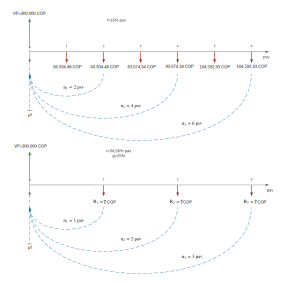
\includegraphics[trim=-78 -5 -78 -5]{7_Capitulo/img/ejemplos/8/8_3.pdf} }   \\ \hline
			%%%%% INICIO FLUJO DE CAJA
			\rowcolor[HTML]{FFB183}
			\multicolumn{2}{|c|}{\cellcolor[HTML]{FFB183}\textbf{4. Declaración de fórmulas}} \\ \hline
			%%%%%%%%%%%%% FIN INSERCIÓN DE IMAGEN
			%%%%%FIN FLUJO DE CAJA
		
			\multicolumn{2}{|c|}{ $VP = \frac{R( (1 + g)^{n} (1+i)^{-n} - 1)}{g-i} $ Valor presente gradiente geométrico}   \\  \hline
			
			%%%%%% INICIO DESARROLLO MATEMÁTICO
			\rowcolor[HTML]{FFB183}
			%%%%%%%%%%INICIO TITULO
			\multicolumn{2}{|c|}{\cellcolor[HTML]{FFB183}\textbf{5. Desarrollo matemático}}       \\ \hline
			%%%%%%%%%% FIN TITULO
			%%%%%%%%%% INICIO MATEMÁTICAS
			\multicolumn{2}{|c|}{  $300.000 \ COP = \frac{R_{1}( (1 + 0,25)^{3} (1+0,3456)^{-3} - 1)}{0,25-0,3456} $}   \\ 
			\multicolumn{2}{|c|}{ $ R_{1} = 225.920,73 \ COP $ }   \\ \hline
			
			%%%%%%%%%% FIN MATEMÁTICAS
			%%%%%% FIN DESARROLLO MATEMÁTICO
			%%%%%% INICIO RESPUESTA
			\rowcolor[HTML]{FFB183}
			%%%%%%%%%%INICIO TITULO
			\multicolumn{2}{|c|}{\cellcolor[HTML]{FFB183}\textbf{6. Respuesta}}   \\ \hline
			%%%%%%%%%% FIN TITULO
			%%%%%%%%%% INICIO RESPUESTA MATEMÁTICA
			\multicolumn{2}{|c|}{ 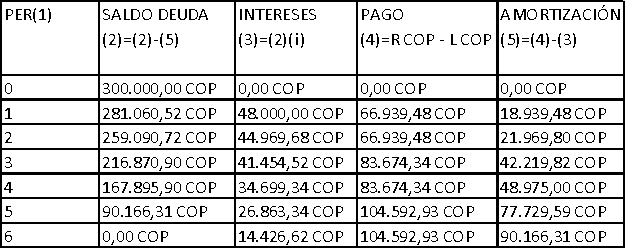
\includegraphics[trim=-78 -5 -78 -5]{7_Capitulo/img/ejemplos/8/8_3_3.pdf} }   \\ \hline
			%\multicolumn{2}{|C{\textwidth}|}{
			%	$R_{58} =  COP  72.478,16(1 + 0,02)^{57} =  COP  224.087,15 $ 
			%}  \\ \hline
			
			
			%%%%%%%%%% FIN MATEMÁTICAS
			%%%%%% FIN RESPUESTA
		\end{longtable}
		%Se crean dos lineas en blanco para que no quede el siguiente texto tan pegado
		%\newline \newline %USARLO SI CREES QUE ES NECESARIO
	\end{center}
 %%%%%%%%%%%%%%%%%%%%%%%%%%FIN EJERCICIO 8c %%%%%%%%%%%%%%%%%%%%%%%%%%%
    %%%%%%%%%%%%%%%%%%%%%%%%%%FIN EJERCICIO 8c %%%%%%%%%%%%%%%%%%%%%%%%%%%

%%%%%%%%%%%%%%%%%%%%%%%%%%FIN EJERCICIO 8 %%%%%%%%%%%%%%%%%%%%%%%%%%%
%%%%%%%%%% NO OLVIDAR COLOCAR ESTE COMENTARIO CON EL NUMERO DE EJERCICIO %%%%%%%%%%%%%
%%%%%%%%%%%%%%%%%%% EJERCICIO 9 %%%%%%
%%Text bf para negrilla , el \\ es para el salto de linea.
%%El primer \\ hace un espacio en el texto y el 2 \\ crea otro espacio
\textbf{Ejemplo 7}\newline
Elaborar una tabla para amortizar la suma de 10.000.000 COP en 4 pagos iguales, suponiendo una tasa de interés de 40\% nominal anual trimestre vencido.\\ \\

\textbf{Solución.}\\
\begin{center}

    \renewcommand{\arraystretch}{1.5}% Margenes de las celdas
    %Creación de la cuadricula
    \begin{longtable}{|c|c|c| }
        %Creamos una linea horizontal
        \hline
        %Definimos el color de la primera fila
        \rowcolor[HTML]{FFB183}
        %%%%% INICIO ASIGNACIÓN FECHA FOCAL %%%%%%%
        %%%%%%%%%% INICIO TITULO
        %Lo que se hace aquí es mezclar las 3 columnas en una sola
        \multicolumn{3}{|c|}{\cellcolor[HTML]{FFB183}\textbf{1. Asignación período focal}}   \\ \hline
        %%%%%%%%%% FIN TITULO
        %%%%% INICIO DECLARACIÓN DE VARIABLES %%%%%%%
        \multicolumn{3}{|c|}{$pf = 0 ptv$} \\ \hline
        %Definimos el color de la primera fila
        \rowcolor[HTML]{FFB183}
        %%%%% INICIO DECLARACIÓN DE VARIABLES %%%%%%%
        %%%%%%%%%% INICIO TITULO
        \multicolumn{3}{|c|}{\cellcolor[HTML]{FFB183}\textbf{2. Declaración de variables}}      \\ \hline
        %%%%%%%%%% FIN TITULO
        %%%%%%%%%% INICIO DE MATEMÁTICAS
        \multicolumn{3}{|c|}{$j=40\% natv \equiv 10\% ptv =i$}\\ \hline
        $n=4$  ptv & $VP =$ 10.000.000 COP & $R= ? COP $                                                                     \\ \hline

        %%%%%%%%%% FIN DE MATEMÁTICAS
        %%%%% FIN DECLARACIÓN DE VARIABLES


        %%%%% INICIO FLUJO DE CAJA
        \rowcolor[HTML]{FFB183}
        \multicolumn{3}{|c|}{\cellcolor[HTML]{FFB183}\textbf{3. Diagrama de flujo de caja}}         \\ \hline
        %Mezclamos 3 columnas y pondremos el dibujo
        %%%%%%%%%%%%% INSERCIÓN DE LA IMAGEN
        \multicolumn{3}{|c|}{ \includegraphics[scale=1]{4_Capitulo/img/ejemplos/9/capitulo4ejemplo9.pdf} } \\ \hline 
        %%%%%%%%%%%%% FIN INSERCIÓN DE IMAGEN
        %%%%%FIN FLUJO DE CAJA



        %%%%% INICIO DECLARACIÓN FORMULAS
        %%%%%%%%%%% INICIO TITULO
        \rowcolor[HTML]{FFB183}
        \multicolumn{3}{|c|}{\cellcolor[HTML]{FFB183}\textbf{4. Declaración de fórmulas}}       \\ \hline
        %%%%%%%%%%% FIN TITULO
        %%%%%%%%%%% INICIO MATEMÁTICAS

        \multicolumn{3}{|c|}{$VP=R\frac{(1-(1+i)^{-n})}{i}$ Valor presente serie uniforme vencida}  \\ \hline
        %%%%%%%%%% FIN MATEMÁTICAS
        %%%%%% INICIO DESARROLLO MATEMÁTICO
        \rowcolor[HTML]{FFB183}
        %%%%%%%%%%INICIO TITULO
        \multicolumn{3}{|c|}{\cellcolor[HTML]{FFB183}\textbf{5. Desarrollo matemático}}    \\ \hline
        %%%%%%%%%% FIN TITULO
        %%%%%%%%%% INICIO MATEMÁTICAS
        \multicolumn{3}{|c|}{10.000.000 COP$=R\frac{(1-(1+0,1)^{-4})}{0,1}$ }     \\ \hline
        %%%%%%%%%% FIN MATEMÁTICAS
        %%%%%% FIN DESARROLLO MATEMÁTICO

        \rowcolor[HTML]{FFB183}
        \multicolumn{3}{|c|}{\cellcolor[HTML]{FFB183}\textbf{6. Respuesta}}    \\ \hline

        \multicolumn{3}{|c|}{R=3.154.708 COP} \\ \hline
        \multicolumn{3}{|c|}{ \includegraphics[scale=0.8]{4_Capitulo/img/ejemplos/9/Capitulo4Ejemplo9Solucion.pdf} } \\ \hline      
    \end{longtable}
    %Se crean dos lineas en blanco para que no quede el siguiente texto tan pegado
    %\newline \newline
\end{center}
%%%%%%%%%%%%%%%%%%%%%%%%%%FIN EJERCICIO X %%%%%%%%%%%%%%%%%%%%%%%%%%%

\newpage
	\textbf{Ejemplo 10}\newline
Supongamos que faltando 10 días para el vencimiento el inversionista del ejemplo anterior decide venderlo y para esta época se están negociando en Bolsa con una tasa del 28\% período 10 días vencido, por lo tanto la tasa de registro debe ser del 28\% período 10 días Vencido. El valor de compra del ejemplo anterior es de 97,204\% COP (faltando 40 días) Suponer el año de 365 días. Calcular:\\
1. El precio de registro en bolsa. \\
2. La retención en la fuente que debe reconocer al vendedor. \\
3. La tasa del vendedor. \\
4. El precio de vendedor. \\
5. Valor de venta.  \\
6. Tasa del comprador. \\
7. Valor del comprador. \newline
\textbf{Solución.
\newline}
\begin{center}
    \renewcommand{\arraystretch}{1.5}% Margenes de las celdas
    %Creación de la cuadricula
    \begin{longtable}[H]{|c|c|c| }
        %Creamos una linea horizontal
        \hline
        %Definimos el color de la primera fila
        \rowcolor[HTML]{FFB183}
        %%%%% INICIO ASIGNACIÓN FECHA FOCAL %%%%%%%
        %%%%%%%%%% INICIO TITULO
        %Lo que se hace aquí es mezclar las 3 columnas en una sola
        \multicolumn{3}{|c|}{\cellcolor[HTML]{FFB183}\textbf{1. Asignación período focal}}   \\ \hline
        %%%%%%%%%% FIN TITULO
        %%%%% INICIO DECLARACIÓN DE VARIABLES %%%%%%%
        \multicolumn{3}{|c|}{$pf = 10 pdv $} \\ \hline
        %Definimos el color de la primera fila
        \rowcolor[HTML]{FFB183}
        %%%%% INICIO DECLARACIÓN DE VARIABLES %%%%%%%
        %%%%%%%%%% INICIO TITULO
        \multicolumn{3}{|c|}{\cellcolor[HTML]{FFB183}\textbf{2. Declaración de variables}}                                                                                   \\ \hline
        %%%%%%%%%% FIN TITULO
        %%%%%%%%%% INICIO DE MATEMÁTICAS
        $F =  100 COP  $ & 
        \multicolumn{2}{c|}{$ a) P_{r} =  ? COP;$\hspace{0.5cm}$ b) i_{v} =  ? \% pdv $} \\
        $ n = 10/365 = 0,027 pdv $ &
        \multicolumn{2}{c|}{$ c) P_{v} = ? COP;$\hspace{0.5cm}$ d) V_{v} =  ? COP $} \\
        $ n = (40-10)/365 pdv $ &
        \multicolumn{2}{c|}{ $ e) i_{c} = ? \% pdv;$\hspace{0.5cm}$ f) P_{c} = ? COP $ } \\
        $ i_{r} = 28\% 10 pdv $     & 
        \multicolumn{2}{c|}{ $ g) V_{c} = ? COP;$\hspace{0.5cm}$ h) R_{F} = ? COP $ } \\
        $ P_{c1} =  97,204 COP $   & 
        \multicolumn{2}{c|}{ $  $ }
        \\ \hline
        %%%%%%%%%% FIN DE MATEMÁTICAS
        %%%%% FIN DECLARACIÓN DE VARIABLES
        
        
        %%%%% INICIO FLUJO DE CAJA
        \rowcolor[HTML]{FFB183}
        \multicolumn{3}{|c|}{\cellcolor[HTML]{FFB183}\textbf{3. Diagrama de flujo de caja}}                                                                                  \\ \hline
        %Mezclamos 3 columnas y pondremos el dibujo
        %%%%%%%%%%%%% INSERCIÓN DE LA IMAGEN
\multicolumn{2}{|c|}{ 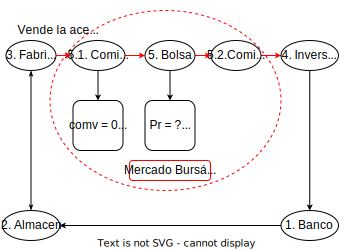
\includegraphics[trim=-90 -5 -90 -5]{3_Capitulo/img/ejemplos/10/capitulo3ejercicio10.pdf} }                                                                                      \\ \hline
        %%%%%%%%%%%%% FIN INSERCIÓN DE IMAGEN
        %%%%%FIN FLUJO DE CAJA
        
        
        
        %%%%% INICIO DECLARACIÓN FORMULAS
        %%%%%%%%%%% INICIO TITULO
        \rowcolor[HTML]{FFB183}
        \multicolumn{3}{|c|}{\cellcolor[HTML]{FFB183}\textbf{4. Declaración de fórmulas}}                                                                                    \\ \hline
        %%%%%%%%%%% FIN TITULO
        %%%%%%%%%%% INICIO MATEMÁTICAS
    
         \multicolumn{3}{|c|}{$P=F(1+i)^{-n}$\hspace{35pt}\textit{Valor presente}
         \hspace{0.3cm}}\\
         \multicolumn{3}{|c|}{$R_{F} = (F - P)*0,7$\hspace{35pt}\textit{Retención en la fuente}
         \hspace{0.3cm}}\\
         \multicolumn{3}{|c|}{$V_{V} = P_{V} * V_{total}$\hspace{35pt}\textit{}
         \hspace{0.3cm}}\\
         \multicolumn{3}{|c|}{$V_{C} = P_{C} * V_{total}$\hspace{35pt}\textit{}
         \hspace{0.3cm}}\\
        
         
         \hline
        %%%%%%%%%% FIN MATEMÁTICAS
        %%%%%% INICIO DESARROLLO MATEMÁTICO
        \rowcolor[HTML]{FFB183}
        %%%%%%%%%%INICIO TITULO
        \multicolumn{3}{|c|}{\cellcolor[HTML]{FFB183}\textbf{5. Desarrollo matemático}}                                                                                      \\ \hline
        %%%%%%%%%% FIN TITULO
        %%%%%%%%%% INICIO MATEMÁTICAS
         \multicolumn{3}{|c|}{$ a) P_{r} = 100 COP * (1 + 0,28)^{-10/365} = 99,3260\% COP$
         \hspace{0.3cm}}\\
         \multicolumn{3}{|c|}{$ b) 97,204 COP = 99.3260 (1+i)^{-30/365} => i_{v} = 6,4\% pdv$
         \hspace{0.3cm}}\\
         \multicolumn{3}{|c|}{$ d) V_{v} = 0,972 COP * 5{.}000{.}000 COP = 4{.}860{.}000 COP $
         \hspace{0.3cm}}\\
         \multicolumn{3}{|c|}{$ e) 99,3260 \% = 100 COP (1+ i)^{-10/365} => i = 9,84\%$
         \hspace{0.3cm}}\\
         \multicolumn{3}{|c|}{$ f) P_{c} = 100 COP (1 + 0,0984)^{-10/365} = 90,16\% COP $
         \hspace{0.3cm}}\\
         \multicolumn{3}{|c|}{$ g) V_{c} = 0,9016 * 5{.}000{.}000 COP = 4{.}508{.}000 COP $
         \hspace{0.3cm}}\\
         \multicolumn{3}{|c|}{$ h) R_{F} = 0,07(5{.}000{.}000 - 97,204) $
         \hspace{0.3cm}}\\
         
        %%%%%%%%%% FIN MATEMÁTICAS
        %%%%%% FIN DESARROLLO MATEMÁTICO
        
        \rowcolor[HTML]{FFB183}
        \multicolumn{3}{|c|}{\cellcolor[HTML]{FFB183}\textbf{6. Respuesta}} \\ \hline    
        
        \multicolumn{3}{|c|}{$P_{r} = 4{.}964{.}190 COP $} \\ \hline
    \end{longtable}
    %Se crean dos lineas en blanco para que no quede el siguiente texto tan pegado
\end{center}

\textbf{Ejemplo 11}\\
Se hacen depósitos trimestrales con incremento del 5\% entre flujos, en una cuenta que paga el 5,25\% periódica trimestral vencida, con el fin de tener disponibles 500.000 COP el primero de enero de 1991, Si el primer depósito se hace el primero de abril de 1988 y el último el primero de julio de 1990, determinar el valor del primer depósito:\\

	%%%%%%%%%%%%%%%%%%% EJERCICIO 11 %%%%%%

%\newpage %USAR SOLO SI EL SOLUCIÓN QUEDA SOLO Y ES NECESARIO BAJARLO A LA SIGUIENTE PAGINA
\textbf{Solución.}\\
%La tabla ira centrada
\begin{center}
	\renewcommand{\arraystretch}{1.6}% Margenes de las celdas
	%Creación de la cuadricula de 3 columnas
	\begin{longtable}[H]{|c|c|c|}
		%Creamos una linea horizontal
		\hline
		%Definimos el color de la primera fila
		\rowcolor[HTML]{FFB183}
		%%%%% INICIO ASIGNACIÓN FECHA FOCAL %%%%%%%
		%%%%%%%%%% INICIO TITULO
		%Lo que se hace aquí es mezclar las 3 columnas en una sola
		\multicolumn{3}{|c|}{\cellcolor[HTML]{FFB183}\textbf{1. Asignación período focal}}  \\ \hline
		\multicolumn{3}{|c|}{$pf = \textit{12 ptv}$}   \\\hline
		%%%%%%%%%% FIN TITULO
		%%%%% INICIO DECLARACIÓN DE VARIABLES %%%%%%%
		%%%%%%%%%% INICIO TITULO
		%Lo que se hace aquí es mezclar las 3 columnas en una sola
		\multicolumn{3}{|c|}{\cellcolor[HTML]{FFB183}\textbf{2. Declaración de variables}}   \\ \hline
		%%%%%%%%%% FIN TITULO
		%%%%%%%%%% INICIO DE MATEMÁTICAS
		%Cada & hace referencia al paso de la siguiente columna
		\multicolumn{2}{|c|}{$\hspace{2 cm}VP=  500{.}000 COP \hspace{2 cm}$} & $i=5.25\% \textit{ ptv}$ \\
		\multicolumn{2}{|c|}{$\hspace{2 cm}n_1=10  \textit{ pav} \hspace{2 cm}$} & $g=5\% \textit{crecimiento geométrico periódico } $ \\
		\multicolumn{2}{|c|}{$\hspace{2 cm}n_2=2  \textit{ pav} \hspace{2 cm}$} & $R= ?COP $ \\ \hline	
		
		%%%%%%%%%% FIN DE MATEMÁTICAS
		%%%%% FIN DECLARACIÓN DE VARIABLES
		
		%%%%% INICIO FLUJO DE CAJA
		\rowcolor[HTML]{FFB183}
		\multicolumn{3}{|c|}{\cellcolor[HTML]{FFB183}\textbf{3. Diagrama de flujo de caja}} \\ \hline
		%Mezclamos 3 columnas y pondremos el dibujo
		%%%%%%%%%%%%% INSERCIÓN DE LA IMAGEN
		%Deberán descargar las imágenes respectivas del drive y pegarlas en la carpeta
		%n_capitulo/img/ejemplos/1/capitulo1ejemplo1.pdf  (el /1/ es el numero del ejemplo)
		\multicolumn{3}{|c|}{ \includegraphics[trim=-5 -5 -5 -5 , scale=0.8]{6_Capitulo/img/ejemplos/11/Capitulo6Ejemplo11.pdf} }
		\\ \hline
		%%%%%%%%%%%%% FIN INSERCIÓN DE IMAGEN
		%%%%%FIN FLUJO DE CAJA
		
		%%%%% INICIO DECLARACIÓN FORMULAS
		%%%%%%%%%%% INICIO TITULO
		\rowcolor[HTML]{FFB183}
		\multicolumn{3}{|c|}{\cellcolor[HTML]{FFB183}\textbf{4. Declaración de fórmulas}}    \\ \hline
		%%%%%%%%%%% FIN TITULO
		%%%%%%%%%%% INICIO MATEMÁTICAS
		\multicolumn{3}{|c|}{$VF=(\frac{(R)[(1+g)^{n}-(1+i)^{n}]}{g-i}) \hspace{0.4 cm} \textit{Valor futuro gradiente si } g \neq i $} \\  
		\multicolumn{3}{|c|}{$F=P(1+i)^{n} \hspace{0.4 cm} \textit{Valor futuro}$} \\ \hline
		
		%%%%%%%%%% FIN MATEMÁTICAS
		%%%%%% INICIO DESARROLLO MATEMÁTICO
		\rowcolor[HTML]{FFB183}
		%%%%%%%%%%INICIO TITULO
		\multicolumn{3}{|c|}{\cellcolor[HTML]{FFB183}\textbf{5. Desarrollo matemático}}       \\ \hline
		%%%%%%%%%% FIN TITULO
		%%%%%%%%%% INICIO MATEMÁTICAS
		\multicolumn{3}{|c|}{$ 500{.}000COP=\frac{(R)[(1-0.05)^{10}-(1+0.0525)^{-10}]}{0.5-0.0525} \cdot (1+0.0525)^{2}  \hspace{0.4 cm} $} \\ \hline
		%%%%%%%%%% FIN MATEMÁTICAS
		%%%%%% FIN DESARROLLO MATEMÁTICO
		%%%%%% INICIO RESPUESTA
		\rowcolor[HTML]{FFB183}
		%%%%%%%%%%INICIO TITULO
		\multicolumn{3}{|c|}{\cellcolor[HTML]{FFB183}\textbf{6. Respuesta}}   \\ \hline
		%%%%%%%%%% FIN TITULO
		%%%%%%%%%% INICIO RESPUESTA MATEMÁTICA
		\multicolumn{3}{|c|}{${R=  72{.}468.80COP}$} \\ \hline
		%%%%%%%%%% FIN MATEMÁTICAS
		%%%%%% FIN RESPUESTA
	\end{longtable}
	%Se crean dos lineas en blanco para que no quede el siguiente texto tan pegado
	%\newline \newline %USARLO SI CREES QUE ES NECESARIO
\end{center}

%%%%%%%%%%%%%%%%%%%%%%%%%%FIN EJERCICIO 11 %%%%%%%%%%%%%%%%%%%%%%%%%%%

%%%%%%%%%%%%%%%%%%% EJERCICIO 12 %%%%%%
\textbf{Ejemplo 12}\\
Una deuda de 15.000 COP fue contraída hace 2 meses con fecha de vencimiento en 4
meses a partir de hoy, esta posee un interés del 24\% nominal anual trimestre vencido y
otra deuda de 25.000 COP contraída hace un mes con vencimiento de 8 meses a partir de hoy
e intereses del 28\% nominal anual semestre vencido. Se van a cancelar las deudas
mediante dos pagos de igual valor, efectuados el primero el día de hoy y el segundo en 6
meses. Con un interés del 30\% nominal anual mes vencido y el segundo en 6 meses,
determinar el valor de los pagos.\\ \\
%\newpage %USAR SOLO SI EL SOLUCIÓN QUEDA SOLO Y ES NECESARIO BAJARLO A LA SIGUIENTE PAGINA
\textbf{Solución.}\\
%La tabla ira centrada
\begin{center}
  \renewcommand{\arraystretch}{1.5}% Margenes de las celdas
  %Creación de la cuadricula de 3 columnas
  \begin{longtable}[H]{|c|c|c|}
    %Creamos una linea horizontal
    \hline
    %Definimos el color de la primera fila
    \rowcolor[HTML]{FFB183}
    %%%%% INICIO ASIGNACIÓN PERíODO FOCAL %%%%%%%
    %%%%%%%%%% INICIO TITULO
    %Lo que se hace aquí es mezclar las 3 columnas en una sola
    \multicolumn{3}{|c|}{\cellcolor[HTML]{FFB183}\textbf{1. Asignación período focal}}                                                                                              \\ \hline
    \multicolumn{3}{|c|}{\textbf{ $pf = \textit{ período focal: 6 pmv} $}}                                                                                                          \\ \hline
    %%%%%%%%%% FIN TITULO
    %%%%% INICIO DECLARACIÓN DE VARIABLES %%%%%%%
    %%%%%%%%%% INICIO TITULO
    %Lo que se hace aquí es mezclar las 3 columnas en una sola
    \multicolumn{3}{|c|}{\cellcolor[HTML]{FFB183}\textbf{2. Declaración de variables}}                                                                                              \\ \hline
    %%%%%%%%%% FIN TITULO
    %%%%%%%%%% INICIO DE MATEMÁTICAS
    %Cada & hace referencia al paso de la siguiente columna
    Deuda 1:                                               & Deuda2:                                                                               & Deuda equivalente              \\
    $j_{1} = 24\% \textit{ natv} $                         & $j_{2} = 28\% \textit{ nasv} $                                                        & $j_{3} = 30\% \textit{ namv} $ \\
    $i_{1} = 6\% \textit{ ptv} $                           & $i_{2} = 14\% \textit{ psv} $                                                         & $i_{3} = 2,5\% \textit{ pmv} $ \\
    $n_ {1} = 2 \textit{ ptv}  $                           & $n_ {2} = 1,5 \textit{ psv} $                                                         & $n_ {3} = 6 \textit{ pmv}  $   \\
    $P_{1} =    15.000 $ COP                               & $P_{2} = 25.000 $ COP                                                              & $F_{5} = F_{6} =  ? $ COP      \\
    $F_{1} =   ? $ COP
    & $F_{2} =   ? $ COP   
    &
    \\
    $F_{3} = ? $ COP
    & $P_{4} = ? $ COP
    &
    \\ \hline


    %%%%%%%%%% FIN DE MATEMÁTICAS
    %%%%% FIN DECLARACIÓN DE VARIABLES


    %%%%% INICIO FLUJO DE CAJA
    \rowcolor[HTML]{FFB183}
    \multicolumn{3}{|c|}{\cellcolor[HTML]{FFB183}\textbf{3. Diagrama de flujo de caja}}                                                                                             \\ \hline
    %Mezclamos 3 columnas y pondremos el dibujo
    %%%%%%%%%%%%% INSERCIÓN DE LA IMAGEN
    %Deberán descargar las imágenes respectivas del drive y pegarlas en la carpeta
    %n_capitulo/img/ejemplos/1/capitulo1ejemplo1.pdf  (el /1/ es el numero del ejemplo)
    \multicolumn{3}{|c|}{ 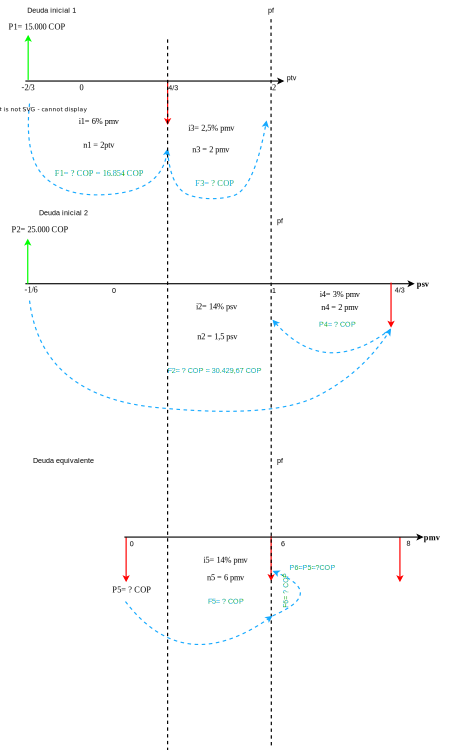
\includegraphics[trim=-5 -5 -5 -5 , scale=0.84]{2_Capitulo/img/ejemplos/14/Ejemplo 12Ver.pdf}}
    \\ \hline
    %%%%%%%%%%%%% FIN INSERCIÓN DE IMAGEN
    %%%%%FIN FLUJO DE CAJA



    %%%%% INICIO DECLARACIÓN FORMULAS
    %%%%%%%%%%% INICIO TITULO
    \rowcolor[HTML]{FFB183}
    \multicolumn{3}{|c|}{\cellcolor[HTML]{FFB183}\textbf{4. Declaración de fórmulas}}                                                                                               \\ \hline
    %%%%%%%%%%% FIN TITULO
    %%%%%%%%%%% INICIO MATEMÁTICAS

    $F = P(1+i)^n \hspace{0.3cm} \textit{Valor futuro}$
    & \multicolumn{2}{c|}{$F_{3}+P_{4}=F_{5}+P_{6}\hspace{0.3cm}\textit{Ecuación de valor}$}
    \\
    $j=i*m\hspace{0.3cm}\textit{Tasa periódica anualizada}$
    & \multicolumn{2}{c|}{$P = F(1+i)^{-n} \hspace{0.3cm} \textit{Valor presente}$ }
 
    \\ \hline

    %%%%%%%%%% FIN MATEMÁTICAS
    %%%%%% INICIO DESARROLLO MATEMÁTICO
    \rowcolor[HTML]{FFB183}
    %%%%%%%%%%INICIO TITULO
    \multicolumn{3}{|c|}{\cellcolor[HTML]{FFB183}\textbf{5. Desarrollo matemático}}                                                                                                 \\ \hline
    %%%%%%%%%% FIN TITULO
    %%%%%%%%%% INICIO MATEMÁTICAS
    $F_{1}= 15.000$ COP $ (1 + 0,06)^{2}=  16.854$ COP    & \multicolumn{2}{|c|}{$16.854$ COP$ (1+0,025)^{2}$}
    \\
    $F_{2}= 25.000$ COP $ (1 + 0,14)^{1,5}= 30.429,67$ COP & \multicolumn{2}{|c|}{$+ 30.429,67$ COP $ (1+0,025)^{-2}$} 
    \\
    &
    \multicolumn{2}{|c|}{$  = P_{5}$ COP $(1+0,025)^{6} + P_{5}$ COP}
    \\
    &
    \multicolumn{2}{|c|}{$P_{5}=21.609,84 $ COP}
    
    \\ \hline


    %%%%%%%%%% FIN MATEMÁTICAS
    %%%%%% FIN DESARROLLO MATEMÁTICO
    %%%%%% INICIO RESPUESTA
    \rowcolor[HTML]{FFB183}
    %%%%%%%%%%INICIO TITULO
    \multicolumn{3}{|c|}{\cellcolor[HTML]{FFB183}\textbf{6. Respuesta}}                                                                                                             \\ \hline
    %%%%%%%%%% FIN TITULO
    %%%%%%%%%% INICIO RESPUESTA MATEMÁTICA
    \multicolumn{3}{|c|}{{$F_{5}$ = $F_{6}$ = 21.609,84 COP.}}                                                                                                                                                                               \\ \hline


    %%%%%%%%%% FIN MATEMÁTICAS
    %%%%%% FIN RESPUESTA
  \end{longtable}
  %Se crean dos lineas en blanco para que no quede el siguiente texto tan pegado
  %\newline \newline %USARLO SI CREES QUE ES NECESARIO
\end{center}
%%%%%%%%%%%%%%%%%%%%%%%%%%FIN EJERCICIO 12 %%%%%%%%%%%%%%%%%%%%%%%%%%%
\setlength{\parskip}{\baselineskip}


\section{Ejercicios propuestos}

En esta sección se dará solución a ejercicios propuestos por los estudiantes
%----------------------------------------------------------------------------------------


%----------------------------------------------------------------------------------------

%\part{Parte Dos}

%----------------------------------------------------------------------------------------
%	CHAPTER 3
%----------------------------------------------------------------------------------------

%\chapterimage{ima2} % Chapter heading image


%Anexos
%\chapter*{Anexos}
%\addcontentsline{toc}{chapter}{\textcolor{ocre}{Anexos}}




%----------------

%----------------------------------------------------------------------------------------
%	BIBLIOGRAPHY
%----------------------------------------------------------------------------------------

%\chapter*{Bibliografía}
%\addcontentsline{toc}{chapter}{\textcolor{ocre}{Bibliografía}}
%\section*{Books}
%\addcontentsline{toc}{section}{Books}
%\printbibliography[heading=bibempty,type=book]



%----------------------------------------------------------------------------------------
%	INDEX
%----------------------------------------------------------------------------------------

\phantomsection
\setlength{\columnsep}{0.75cm}
\printindex

%----------------------------------------------------------------------------------------
% \textbf{Ejemplo 1}\\
% Si invierto hoy un capital de 1.000.000 COP, cuánto capital podré retirar en 18 meses suponiendo que el capital invertido gana el 24\% (nasv) nominal anual semeste vencido? \\ \\
% %\newpage %USAR SOLO SI EL SOLUCIÓN QUEDA SOLO Y ES NECESARIO BAJARLO A LA SIGUIENTE PAGINA
% \textbf{Solución.}\\
% %La tabla irá centrada
% \begin{center}
%  \renewcommand{\arraystretch}{1.5}% Margenes de las celdas
%  %Creación de la cuadricula de 3 columnas
%  \begin{longtable}[H]{|p{0.5\linewidth}|p{0.5\linewidth}|}
%   \hline
%   \multicolumn{2}{|c|}{\cellcolor[HTML]{FFB183}\textbf{1. Declaración de variables}}                  \\ \hline
%   $n = 3 \hspace{1mm} psv$                                      & $VF =  1{.}000{.}000$ COP             \\
%   $j = 24\% \hspace{1mm} nasv \equiv i = 12\% \hspace{1mm} psv$ & $VP =  ?$ COP                       \\ \hline
%   \multicolumn{2}{|c|}{\cellcolor[HTML]{FFB183}\textbf{2. Tabla de flujo de caja}}                    \\ \hline
%   \multicolumn{2}{|p{\columnwidth}|}{
%   \begin{center}
%    \begin{tabular}{|c|c|}
%     \hline
%     Periodo (psv) & Flujo          \\ \hline
%     $0$           &  1.000.000 COP             \\ \hline
%     $1$           &  COP -            \\ \hline
%     $2$           &  COP -            \\ \hline
%     $3$           &  ? COP \\ \hline
%    \end{tabular}
%   \end{center}
%   }                                                                                                   \\ \hline
%   \multicolumn{2}{|c|}{\cellcolor[HTML]{FFB183}\textbf{3. Fórmulas utilizadas}}                       \\ \hline
%   \multicolumn{2}{|l|}{Mediante el uso de Excel:}                                                     \\
%   \multicolumn{2}{|l|}{VF (Valor futuro): Devuelve el valor futuro para una inversión}              \\ \hline
%   \multicolumn{2}{|c|}{\cellcolor[HTML]{FFB183}\textbf{4. Desarrollo en Excel}}                       \\ \hline
%   \multicolumn{2}{|l|}{Se aplicará la función VF de la siguiente forma:}                              \\
%   \multicolumn{2}{|c|}{ \includegraphics[trim=-5 -5 -5 -5 ,width=1\columnwidth]{1/Ejem1.PNG}}         \\
%   \multicolumn{2}{|l|}{=VA (0,12; 18; -1000000) con referencia en la hoja de Excel usada para el ejercicio.} \\ \hline
%   \multicolumn{2}{|c|}{\cellcolor[HTML]{FFB183}\textbf{5. Respuesta}}                                 \\ \hline
%   \multicolumn{2}{|c|}{El valor futuro (VF) es de  7.689.965 COP.}               \\ \hline
%   \multicolumn{2}{|c|}{\cellcolor[HTML]{FFB183}\textbf{6. Gráfica}}                                   \\ \hline
%   \multicolumn{2}{|c|}{No es necesaria la realización de una gráfica para este ejercicio.}            \\ \hline
%  \end{longtable}
%  %\newline \newline %USARLO SI CREES QUE ES NECESARIO
% \end{center}

% \textbf{Ejemplo 2}\\
% Dado el 24\% periodo 3 años vencido, hallar una tasa periódica equivalente para periodo 2 años vencido\\ \\
% %\newpage %USAR SOLO SI EL SOLUCIÓN QUEDA SOLO Y ES NECESARIO BAJARLO A LA SIGUIENTE PAGINA
% \textbf{Solución.}\\
% %La tabla irá centrada
% \begin{center}
%  \renewcommand{\arraystretch}{1.5}% Margenes de las celdas
%  %Creación de la cuadricula de 3 columnas
%  \begin{longtable}[H]{|p{0.5\linewidth}|p{0.5\linewidth}|}
%   \hline
%   \multicolumn{2}{|c|}{\cellcolor[HTML]{FFB183}\textbf{1. Declaración de variables}}                         \\ \hline
%   \multicolumn{1}{|c|}{$m=\frac{3}{2}p(2a)v$  $T=8\% $ na$i_1=24\% p(3a)v$  $i_2=?\% p(2a)v$ }              \\ \hline                                         
%   \multicolumn{2}{|c|}{\cellcolor[HTML]{FFB183}\textbf{2. Tabla de flujo de caja}}                           \\ \hline
%   \multicolumn{2}{|c|}{En este ejercicio, no se realiza la tabla de flujo de caja.}                          \\ \hline
%   \multicolumn{2}{|c|}{\cellcolor[HTML]{FFB183}\textbf{3. Fórmulas utilizadas}}                              \\ \hline
%   \multicolumn{2}{|l|}{Mediante el uso de Excel:}                                                            \\
%   \multicolumn{2}{|l|}{INT.EFECTIVO: Devuelve la tasa de interés anual efectiva}                             \\ \hline
%   \multicolumn{2}{|c|}{\cellcolor[HTML]{FFB183}\textbf{4. Desarrollo en Excel}}                              \\ \hline
% \multicolumn{2}{|l|}{Se aplicará la función INT.EFECTIVO de la siguiente forma:}                             \\
%   \multicolumn{2}{|c|}{ \includegraphics[trim=-5 -5 -5 -5 ,width=1\columnwidth]{2/Ejem2.1.PNG}}              \\
%   \multicolumn{2}{|c|}{ \includegraphics[trim=-5 -5 -5 -5 ,width=1\columnwidth]{2/Ejem2.2.PNG}}
%  \\ \hline
%   \multicolumn{2}{|c|}{\cellcolor[HTML]{FFB183}\textbf{5. Respuesta}}                                        \\ \hline
%   \multicolumn{2}{|c|}{La tasa es del 16,11\% período 2 año vencido}                                        \\ \hline
%   \multicolumn{2}{|c|}{\cellcolor[HTML]{FFB183}\textbf{6. Gráfica}}                                          \\ \hline
%   \multicolumn{2}{|c|}{No es necesaria la realización de una gráfica para este ejercicio.}                   \\ \hline
%  \end{longtable}
%  %\newline \newline %USARLO SI CREES QUE ES NECESARIO
% \end{center}

% \textbf{Ejemplo 3}\\
% \vspace{2mm}

% Una persona tiene dos deudas una de  250.000 COP pagadera en 3 meses y otra de 400.000  COP pagadera en 7 meses. Si desea cambiar la forma de cancelarlas mediante dos pagos iguales de X COP cada uno con vencimiento en 5 meses y 12 meses respectivamente, determinar el valor de los pagos suponiendo una tasa del 24\% (namv) nominal anual mes vencido.\\ \\
% %\newpage %USAR SOLO SI EL SOLUCIÓN QUEDA SOLO Y ES NECESARIO BAJARLO A LA SIGUIENTE PAGINA
% \textbf{Solución.}\\
% %La tabla irá centrada
% \begin{center}
%  \renewcommand{\arraystretch}{1.5}% Margenes de las celdas
%  %Creación de la cuadricula de 3 columnas
%  \begin{longtable}[H]{|p{0.5\linewidth}|p{0.5\linewidth}|}
%   \hline
%   \multicolumn{2}{|c|}{\cellcolor[HTML]{FFB183}\textbf{1. Declaración de variables}}                          \\ \hline
%   Deuda Inicial      & Deuda equivalente                                                                      \\
%   $D_1= 250.000 COP $ & $n_1 = 5 pmv$                                                                          \\
%   $n_1=3 pmv$        & $n_2 = 10 pmv$                                                                         \\
%   $D_2= 400.000 COP $ & $j = 24 \% namv$                                                                     \\
%   $n_2=7 pmv$        & $i = 2 \% pmv$                                                                        \\ \hline
%   \multicolumn{2}{|c|}{\cellcolor[HTML]{FFB183}\textbf{2. Tabla de flujo de caja}}                            \\ \hline
%   \multicolumn{2}{|p{\columnwidth}|}{
%   \begin{center}
%    \begin{tabular}{|p{4cm}|p{4cm}|p{4cm}|}
%     \hline
%     \textbf{Periodo} & \textbf{Deuda Inicial} & \textbf{Deuda Equivalente} \\ \hline

%     0                &  COP                      &  COP                          \\ \hline
%     1                &  COP                      &  COP                          \\ \hline
%     2                &  COP                      &  COP                          \\ \hline
%     3                &  250.000 COP              &  COP                          \\ \hline
%     4                &  COP                      &  COP                          \\ \hline
%     5                &  COP                      &  X COP                        \\ \hline
%     6                &  COP                      &  COP                          \\ \hline
%     7                &  400.000 COP              &  COP                          \\ \hline
%     8                &  COP                      &  COP                          \\ \hline
%     9                &  COP                      &  COP                          \\ \hline
%     10               &  COP                      &  COP                          \\ \hline
%     11               &  COP                      &  COP                          \\ \hline
%     12               &  COP                      &  X COP                        \\ \hline
%    \end{tabular}
%   \end{center}
%   }                                                                                                           \\ \hline
%   \multicolumn{2}{|c|}{\cellcolor[HTML]{FFB183}\textbf{3. Fórmulas utilizadas}}                               \\ \hline
%   \multicolumn{2}{|l|}{Mediante el uso de Excel:}                                                             \\
%   \multicolumn{2}{|l|}{VNA (Valor neto actual): Devuelve el valor neto presente de una inversión}                      \\ \hline
%   \multicolumn{2}{|c|}{\cellcolor[HTML]{FFB183}\textbf{4. Desarrollo en Excel}}                               \\ \hline
%   \multicolumn{2}{|l|}{Se aplicará la función VNA de la siguiente forma:}                                      \\
%   \multicolumn{2}{|c|}{ \includegraphics[trim=-5 -5 -5 -5 ,width=1\columnwidth]{3/Ejem3.PNG}}                 \\
%   \multicolumn{2}{|p{\columnwidth}|}{
%   Esta función se aplicará de la siguiente forma en las dos celdas donde se desee obtener
%   el Valor presente de las deudas originales y de las deudas equivalentes.\newline

%   = -VNA(0,02;B7:B19) = -=VNA(0,02;C7:C19)\newline

%   Luego se aplicará la formula Función Objetivo de la siguiente forma:
%   }                                                                                                           \\
%   \multicolumn{2}{|c|}{ \includegraphics[trim=-5 -5 -5 -5 ,width=0.5\columnwidth]{3/Ejem3.2.PNG}} \\ \hline
%   \multicolumn{2}{|c|}{\cellcolor[HTML]{FFB183}\textbf{5. Respuesta}}                                         \\ \hline
%   \multicolumn{2}{|p{\columnwidth}|}{
%   \begin{center}
%    \begin{tabular}{|p{4cm}|p{4cm}|p{4cm}|}
%     \hline
%     \textbf{Periodo} & \textbf{Deuda Inicial} & \textbf{Deuda Equivalente} \\ \hline


%     0                &  COP                      &  COP                          \\ \hline
%     1                &  COP                      &  COP                          \\ \hline
%     2                &  COP                      &  COP                          \\ \hline
%     3                &  25.000,00 COP            &  COP                          \\ \hline
%     4                &  COP                      &  COP                          \\ \hline
%     5                &  COP                      &  35.424,00 COP                \\ \hline
%     6                &  COP                      &  COP                          \\ \hline
%     7                &  40.000,00 COP            &  COP                          \\ \hline
%     8                &  COP                      &  COP                          \\ \hline
%     9                &  COP                      &  COP                          \\ \hline
%     10               &  COP                      &  COP                          \\ \hline
%     11               &  COP                      &  COP                          \\ \hline
%     12               &  COP                      &  35.424,00 COP                \\ \hline
%    \end{tabular}
%   \end{center}

%   Debe realizar dos pagos con el valor de 35.423,66 COP cada uno.
%   }                                                                                                           \\ \hline
%   \multicolumn{2}{|c|}{\cellcolor[HTML]{FFB183}\textbf{6. Gráfica}}                                           \\ \hline
%   \multicolumn{2}{|c|}{No es necesaria la realización de una gráfica para este ejercicio.}                    \\ \hline
%  \end{longtable}
 %\newline \newline %USARLO SI CREES QUE ES NECESARIO
% \end{center}





% \end{document}